\documentclass[letterpaper]{article}
\usepackage{format/aaai}
\usepackage{times}
\usepackage{helvet}
\usepackage{courier}
\frenchspacing
\setlength{\pdfpagewidth}{8.5in}
\setlength{\pdfpageheight}{11in}
\pdfinfo{
/Title (Insert Your Title Here)
/Author (Put All Your Authors Here, Separated by Commas)}
\setcounter{secnumdepth}{0}  



% use Times
%\usepackage{times}
% For figures
\usepackage{graphicx} % more modern
%\usepackage{epsfig} % less modern
\usepackage{subfigure} 

% For citations
%\usepackage{natbib}

% For algorithms
%\usepackage{algorithm}
%\usepackage{algorithmic}
%\usepackage{algorithmicx}

% As of 2011, we use the hyperref package to produce hyperlinks in the
% resulting PDF.  If this breaks your system, please commend out the
% following usepackage line and replace \usepackage{icml2014} with
% \usepackage[nohyperref]{icml2014} above.
%\usepackage{hyperref}

% Packages hyperref and algorithmic misbehave sometimes.  We can fix
% this with the following command.
\usepackage{algorithm}
\usepackage{algorithmic}
\newcommand{\theHalgorithm}{\arabic{algorithm}}

% Employ the following version of the ``usepackage'' statement for
% submitting the draft version of the paper for review.  This will set
% the note in the first column to ``Under review.  Do not distribute.''
%\usepackage{format/icml2014} 
% Employ this version of the ``usepackage'' statement after the paper has
% been accepted, when creating the final version.  This will set the
% note in the first column to ``Proceedings of the...''
%\usepackage[accepted]{icml2014}

%\usepackage{times}
\usepackage{hyperref}
\usepackage{url}
\usepackage{color}
\usepackage{preamble}
\definecolor{mydarkblue}{rgb}{0,0.08,0.45}
\hypersetup{ %
    pdftitle={},
    pdfauthor={},
    pdfsubject={},
    pdfkeywords={},
    pdfborder=0 0 0,
    pdfpagemode=UseNone,
    colorlinks=true,
    linkcolor=mydarkblue,
    citecolor=mydarkblue,
    filecolor=mydarkblue,
    urlcolor=mydarkblue,
    pdfview=FitH}
    
    
\usepackage{amsmath, amsfonts, bm, lipsum, capt-of}
\usepackage{natbib, xcolor, wrapfig, booktabs, multirow, caption}
%\DeclareCaptionType{copyrightbox}
\usepackage{float}
\usepackage{datetime}

%\renewcommand{\baselinestretch}{0.99}

\def\ie{i.e.\ }
\def\eg{e.g.\ }
\let\oldemptyset\emptyset
\let\emptyset 0

\newcommand{\procedurename}{ABCDE}

%\author{
%James Robert Lloyd\\
%University of Cambridge\\
%Department of Engineering\\
%\texttt{jrl44@cam.ac.uk}
%\And
%David Duvenaud\\
%University of Cambridge \\
%Department of Engineering \\
%\texttt{dkd23@cam.ac.uk}
%\And
%Roger Grosse\\
%M.I.T.\\
%Brain and Cognitive Sciences \\
%\texttt{rgrosse@mit.edu}
%\And
%Joshua B. Tenenbaum\\
%M.I.T.\\
%Brain and Cognitive Sciences \\
%\texttt{jbt@mit.edu}
%\And
%Zoubin Ghahramani\\
%University of Cambridge \\
%Department of Engineering \\
%\texttt{zoubin@eng.cam.ac.uk}
%}

\newcommand{\fix}{\marginpar{FIX}}
\newcommand{\new}{\marginpar{NEW}}

\setlength{\marginparwidth}{0.6in}
%%%%%%%%%%%%%%%%%%%%%%%%%%%%%%%%%%%%%%%%%%%%%%%%%%%%%%%%%%
%%%% EDITING HELPER FUNCTIONS  %%%%%%%%%%%%%%%%%%%%%%%%%%%
%%%%%%%%%%%%%%%%%%%%%%%%%%%%%%%%%%%%%%%%%%%%%%%%%%%%%%%%%%

%% NA: needs attention (rough writing whose correctness needs to be verified)
%% TBD: instructions for how to fix a gap ("Describe the propagation by ...")
%% PROBLEM: bug or missing crucial bit 

%% use \fXXX versions of these macros to put additional explanation into a footnote.  
%% The idea is that we don't want to interrupt the flow of the paper or make it 
%% impossible to read because there are a bunch of comments.

%% NA's (and TBDs, those less crucially) should be written so 
%% that they flow with the text.

\definecolor{WowColor}{rgb}{.75,0,.75}
\definecolor{SubtleColor}{rgb}{0,0,.50}

% inline
\newcommand{\NA}[1]{\textcolor{SubtleColor}{ {\tiny \bf ($\star$)} #1}}
\newcommand{\LATER}[1]{\textcolor{SubtleColor}{ {\tiny \bf ($\dagger$)} #1}}
\newcommand{\TBD}[1]{\textcolor{SubtleColor}{ {\tiny \bf (!)} #1}}
\newcommand{\PROBLEM}[1]{\textcolor{WowColor}{ {\bf (!!)} {\bf #1}}}

% as margin notes

\newcounter{margincounter}
\newcommand{\displaycounter}{{\arabic{margincounter}}}
\newcommand{\incdisplaycounter}{{\stepcounter{margincounter}\arabic{margincounter}}}

\newcommand{\fTBD}[1]{\textcolor{SubtleColor}{$\,^{(\incdisplaycounter)}$}\marginpar{\tiny\textcolor{SubtleColor}{ {\tiny $(\displaycounter)$} #1}}}

\newcommand{\fPROBLEM}[1]{\textcolor{WowColor}{$\,^{((\incdisplaycounter))}$}\marginpar{\tiny\textcolor{WowColor}{ {\bf $\mathbf{((\displaycounter))}$} {\bf #1}}}}

\newcommand{\fLATER}[1]{\textcolor{SubtleColor}{$\,^{(\incdisplaycounter\dagger)}$}\marginpar{\tiny\textcolor{SubtleColor}{ {\tiny $(\displaycounter\dagger)$} #1}}}


%% For submission, make all render blank.
%\renewcommand{\LATER}[1]{}
%\renewcommand{\fLATER}[1]{}
%\renewcommand{\TBD}[1]{}
%\renewcommand{\fTBD}[1]{}
%\renewcommand{\PROBLEM}[1]{}
%\renewcommand{\fPROBLEM}[1]{}
%\renewcommand{\NA}[1]{#1}  % Note, NA's pass through!


% The \icmltitle you define below is probably too long as a header.
% Therefore, a short form for the running title is supplied here:
%\icmltitlerunning{Automatic construction and natural-language description of nonparametric regression models}

\setcounter{secnumdepth}{2}

 \begin{document}
% The file aaai.sty is the style file for AAAI Press 
% proceedings, working notes, and technical reports.
%
\title{Automatic Construction and Natural-language Description \\ of Nonparametric Regression Models}
\author{}
\maketitle


%\twocolumn[
%\icmltitle{Automatic Construction and Natural-language Description \\ of Nonparametric Regression Models
%}

% It is OKAY to include author information, even for blind
% submissions: the style file will automatically remove it for you
% unless you've provided the [accepted] option to the icml2014
% package.
%\icmlauthor{Your Name}{email@yourdomain.edu}
%\icmladdress{Your Fantastic Institute,
%            314159 Pi St., Palo Alto, CA 94306 USA}
%\icmlauthor{Your CoAuthor's Name}{email@coauthordomain.edu}
%\icmladdress{Their Fantastic Institute,
%            27182 Exp St., Toronto, ON M6H 2T1 CANADA}

% You may provide any keywords that you 
% find helpful for describing your paper; these are used to populate 
% the "keywords" metadata in the PDF but will not be shown in the document
%\icmlkeywords{}

%\vskip 0.3in
%]

\begin{abstract} 
%Compiled on \today\ at \currenttime
%\\
This paper presents the beginnings of an automatic statistician, which has the potential to aid in exploratory analysis of data.
Specifically, we develop a nonparametric model construction procedure which also automatically produces natural-language descriptions of the model.
The procedure takes a data set as input, runs an open-ended model search and then produces a detailed report with figures and text which decompose and describe the various patterns discovered.
We describe how the Gaussian process models being searched over naturally decompose into interpretable structures, which allow simple rule-based descriptions of arbitrarily complex models.
The procedure contains many standard regression techniques as special cases, leading to superior extrapolation ability.
\end{abstract} 

%\allowdisplaybreaks

\section{Introduction}
%One aim of statistics is to produce accurate and concise descriptions of data which yield insight into underlying sources of variability.
%This requires the construction and fitting of an appropriate statistical model that can be interpreted by the user.
%For some simple model classes, such as linear regression, there already exist standard software packages which automatically fit the model and report results to the user.

%Simple parametric regression models such as linear regression are usually easy to interpret, requiring only a table of regression coefficients and a few other parameters to describe a model.
%However, simple parametric models such as linear regression may often be too simple to accurately describe many data sets.
One aim of statistics is to produce accurate and concise descriptions of data which yield insight into underlying sources of variability.
%Many datasets are too complex to be accurately described by simple parametric models such as linear regression.
Non-parametric regression models such as Gaussian processes are flexible enough to model complex nonlinear phenomena. Unfortunately, their design and interpretation can require considerable human time and expertise, and the results are inevitably filtered through the preconceived notions of the researchers.
%Moreover, non-parametric models can be difficult to summarize, since the fitted parameters (e.g.~bandwidths or typical lengthscales) relate only indirectly to the data.
%with fitted parameters corresponding only to very high level concepts such as bandwidths or typical lengthscales.
%typically require graphical descriptions of their fit, since any text description would be overly simplistic (\eg `a smooth function') and fitted parameters correspond only to very high level concepts such as bandwidths or typical lengthscales.

%Several methods have been proposed for automatically constructing structured nonparametric models from data \citep{diosan2007evolving, bing2010gp, DuvLloGroetal13, kronberger2013evolution}. However, this does not solve the problem of interpretability, as complex kernel structures can obscure the underlying modeling assumptions.
%\citet{DuvLloGroetal13} observed that Gaussian process models could be decomposed into sums of diverse components, and that the different components often corresponded to interpretable features of the data.
%Unfortunately, the outputs of their procedure .
%In that work, components discovered by the automatic model search were interpreted post-hoc by the authors.

Consider what would be required of a system that automates enough of the modeling process to be usable by non-experts and to avoid the biases of human interpretation:
\begin{itemize}
\item {\bf An open-ended language of models} which is expressive enough to capture many of the modeling assumptions and model construction techniques applied by human statisticians
\item {\bf A search procedure} which proposes promising models to fit based on the results of fitting previous models
\item {\bf Methods for evaluating the fit of a model} in terms of the complexity of the model and the degree of fit to the data
\item {\bf Automatic generation of reports} which explain and visualize different factors underlying the data, make explicit the chosen modeling assumptions, and quantify how each component improves the predictive power of the model
\end{itemize}

\begin{figure}[t]
\centering
\fbox{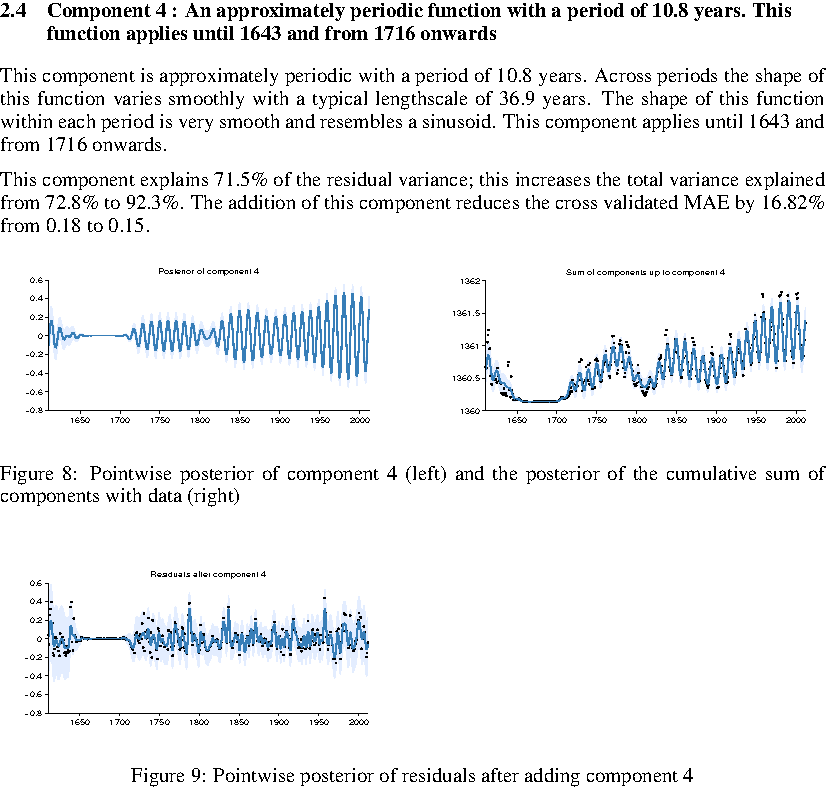
\includegraphics[trim=0cm 4.75cm 0cm 1.0cm, clip, width=0.98\columnwidth]{solarpages/pg_0007-crop}}
\caption{Extract from an automatically-generated report describing the model components discovered by automatic model search.  This part of the report isolates and describes the approximately 11-year sunspot cycle, also noting its disappearance during the 16th century, a time known as the Maunder minumum.}
\label{fig:periodic}
\end{figure}


In this manuscript, we present a procedure which uses the compositional structure of Gaussian process kernels to automatically produce natural-language descriptions of patterns in a data set.
This procedure fulfills all four of the desiderata listed above.
%demonstrate that the compositional structure of Gaussian process models allows for the automatic natural-language description of patterns within a data set.
Given a data set, it runs an open-ended model search and produces a detailed report describing the structures it discovered. % \ie the interpretable models are automatically interpreted!
%
We show examples of automatically generated natural language reports which highlight interpretable features of a variety of data sets.
%This paper contains extracts of the natural-language reports automatically generated by our procedure.
%The text descriptions within these reports clearly communicate interpretable features of the data, supplemented by appropriate figures.
The supplementary material to this paper includes 13 complete reports generated by our method.


%We also\fTBD{RBG: This makes it sound like an independent contribution. Any way to tie it together with the natural language stuff, e.g.~evidence that the changes improve interpretability?} extend and refine the components used in the model construction process to improve the expressivity and interpretability of the models.
%This allows for the procedure to fit and describe many well established modelling motifs including linear regression, Fourier analysis, sparse spectrum \gp{}s \citep{lazaro2010sparse}, changepoints \citep[e.g.][]{garnett2010sequential, FoxDunson:NIPS2012}, heteroscedasiticity, trend-cyclical-irregular \citep[e.g.][]{lind2006basic}\fTBD{Can anyone find a more academic reference?} and multiple kernel learning \citep[e.g.][]{bach2004multiple}.

%Finally, we demonstrate that the extended model construction procedure is comparable or superior to other model construction techniques at extrapolation tasks.
As a test of our procedure's ability to model the underlying structure of a dataset, we compare our procedure against existing model construction techniques on a variety of extrapolation tasks. We find comparable or superior performance. We believe our system is a step towards automating much of the process of model construction, fitting, and analysis, and should allow a broader range of non-experts to fit and interpret nonparametric regression models.




\iffalse

\section{Ingredients of an automatic statistician}
\label{sec:ingredients}
%\fTBD{JL: Has RG written anything on this?}
\citet{gelman2013philblogpost} asks ``How can an artificial intelligence do statistics? ... It needs not just an inference engine, but also a way to construct new models and a way to check models. Currently, those steps are performed by humans, but the AI would have to do it itself.''

%In this section, we discuss in more detail the elements required to build a system that can automatically construct and then describe complex nonparametric models.

In this section, we discuss in more detail the elements we believe are required to build an artificial intelligence that can do statistics.

\paragraph{1. An open-ended language of models}
Many statistical procedures consider all models in a class of fixed size - for example, graphical model construction algorithms\fTBD{Cite} search over connectivity graphs for a given set of nodes.
While these methods can be powerful, human statisticians are capable of deriving novel model classes when required by the modelling task.
%An open ended language can 
An automatic search through an open-ended class of models can achieve some of this flexibility, growing the complexity of the model to fit the task at hand, and possibly combining existing structures in novel ways.
%However, in order for a procedure to be as powerful as a human statistician, it must be able to add to a model in a wide variety of ways, building arbitrarily complex models if the data demands it.

\paragraph{2. Searching through model space}
An open-ended space of models cannot be searched exhaustively.
Just as human researchers iteratively refine their models, search procedures can propose new search directions based on the results of previous model fits.
Because any search in an open-ended space must start with relatively simple models before moving on to more complex ones, any model search in an open-ended space will likely resemble a model-building procedure.% based 

\paragraph{3. Model comparison and checking model fit}
\fTBD{JL: Two sections perhaps - or are they completely intertwined?}
An automatic statistician should be able to question the models it has constructed, and formal procedures from model checking provide a way for it to do this.
%A practically and philsophically interesting question is how to compare models, and how to check whether there is statistical structure not being captured by a given model. 
%\fTBD{Struggling with this section - do we need to defend marginal likelihood or discuss the options}
\citet{gelman2012philosophy} review the literature on model checking.
\TBD{In this work, we use approximate marginal likelihood to compare models, penalizing complexity using the Bayesian Information Criterion as a heuristic.}

\paragraph{4. Describing models}

%Capturing statistical structure helps to provide good predictions. 
Part of the value of statistical models comes from enabling humans to understand a dataset or a phenomenon.
Furthermore, a clear description of the statistical structure found in a dataset helps a user to notice when the dataset has errors, the wrong question was asked, the model-building procedure failed to capture known structure, a relevant piece of data or constraint is missing, or when a novel statistical structure has been found.

%It is not clear\fTBD{JL: Weak} what obstacles there are to building a system capable of explaining novel statistical structures.
In this work, we 
%attempted to build such an automatic summarization procedure, and 
demonstrate that the properties of Gaussian processes allow for a modular description generation procedure.
%This modularity means that a large class of statistical structures can explained, without resorting to writing a special case for every possible structure in our open-ended set of models.
Whether or not such modularity and interpretability is present in other open-ended model classes is an open question.

\fi

\section{A language of regression models}
\label{sec:improvements}



%\subsection{Gaussian processes}

Gaussian processes (\gp{}) \citep{rasmussen38gaussian} are distributions over functions such that the values evaluated at any finite set of points are jointly Gaussian.
Because of their flexibility, they are commonly used for nonparametric regression.
A \gp{} regression model is specified in terms of a kernel function ${\kernel : \mathcal{X}^2 \to \mathbb{R}}$, which defines the covariance between the function values $(\outputVar, \outputVar')$ evaluated at two inputs $(\inputVar,\inputVar')$, \ie ${\textrm{Cov}(\outputVar, \outputVar') = \kernel(\inputVar,\inputVar')}$.
Because the kernel determines which structures are likely under the \gp{} prior, it determines the model's patterns of generalization.

\citet{DuvLloGroetal13} presented a space of Gaussian process kernels defined compositionally through addition and multiplication of a handful of simple kernels.
In this work, we focus on a similar space of models, but with improvements which are discussed in section~\ref{sec:related-work}. 

The buildling blocks of our model space are a handful of ``base'' kernel families with simple parametric forms. Each kernel family has one or more parameters; when the parameters are specified, it defines a kernel function. Each kernel family favors particular kinds of structure; e.g., a \gp{} with a squared-exponential kernel (denoted $\kSE$) favors smooth functions, while a \gp{} with a periodic kernel ($\kPer$) favors periodic functions. The full set of base kernel families is given in Table~{\bf TODO}.

Because the set of kernel functions is closed under addition and multiplication, any algebraic expression consisting of $+$, $\times$, and base kernel families defines a kernel family. 
Such composite kernels can describe richer structures not representable by the base kernels.
For example, the kernel $\kSE \times \kPer$ puts mass on functions which are locally periodic, while a \gp{} with kernel $\kSE + \kLin$ corresponds to a prior on smooth functions with a linear trend. The procedure of \citet{DuvLloGroetal13} automatically searched over the space of composite kernels (represented as algebraic expressions), where the search operators consisted of modifying sub-expressions. 
By combining kernels, the search procedure was able to construct novel nonparametric regression models.
For example, when applied to airline passenger data (see `describing heteroscedasticity'), the resulting kernel contained a component of the form $\kSE \times \kPer \times \kLin$, which captured a feature of the data which can be described as ``approximately periodic, with linearly growing amplitude''.

While the procedure of \citet{DuvLloGroetal13} was able to decompose a variety of datasets into interpretable components, interpreting the final models required human time, expertise, and judgment. Our contribution is a method of automatically generating natural language reports from the outputs of a GP structure search system.
%
We call the entire model-search and description procedure automatic Bayesian covariance decomposition and explanation (\procedurename{}).


%Different kernels can express a wide variety of structures that one might expect to find in functions.
%For example, a \gp{} with a squared-exponential kernel ($\kSE$) corresponds to a prior on smooth functions.
%Similarly, a \gp{} with a periodic kernel ($\kPer$) or linear kernel ($\kLin$) corresponds to a prior on periodic functions or linear functions respectively.
%Definitions of all kernels are provided in the supplementary material.

%\subsection{Compositional model building using kernels}

%To express richer structures, new kernels can be constructed by taking products of existing ones.
%For example, the kernel $\kSE \times \kPer$ puts mass on functions which are locally periodic.
%Additive models can also be constructed by taking sums of kernels.
%For example, a \gp{} with kernel $\kSE + \kLin$ corresponds to a prior on smooth functions with a linear trend.

%These ideas were exploited by \citet{DuvLloGroetal13},  who introduced the Gaussian process structure search procedure (GPSS).
%GPSS searches over sums and products of a set of simple base kernels to produce an appropriate model for a data set.

\iffalse

In the rest of this section we extend the language defined by GPSS to include a greater variety of regression motifs.
We also reparametrise the base kernels resulting in clearer decompositions and descriptions of the models produced.


\subsection{Changepoints}

\gp{}s with hard changepoints have been considered by \citet{garnett2010sequential} and \citet{FoxDunson:NIPS2012}.
We construct soft changepoints by multiplying by sigmoidal functions.
\fTBD{DD: Let's add a small figure here to show what changepoints can do.}
Suppose that $f_1(x) \dist \gp{}(0, \kernel_1)$ and $f_2(x) \dist \gp{}(0, \kernel_2)$ and define
\begin{align}
f(x) = \sigma(x)f_1(x) + (1-\sigma(x)) f_2(x)
\end{align}
where $\sigma(x)$ is a sigmoid function varying between 0 and 1 \ie $f$ transitions between functions $f_1$ and $f_2$.
Then $f(x) \dist \gp{}(0,\kernel)$ where
\begin{align}
\kernel(x,x') = \qquad \qquad \sigma(x) & k_1(x,x')\sigma(x') \nonumber \\ + (1-\sigma(x)) & k_2(x,x')(1-\sigma(x'))
\label{eq:cp}
\end{align}
%(see section~\ref{sec:description} for the properties to prove this identity).
%
We represent this kernel with the changepoint operator $\kCP(\kernel_1, \kernel_2)$.
We also introduce a change window operator, $\kCW(\cdot,\cdot)$, which uses a product of two sigmoids to produce a smooth `hat-shaped' modulation between two functions.

\paragraph{Heteroscedasticity}

We introduce the white noise kernel ($\kWN$) as a base kernel.
Combined with linear kernels and changepoints this can produce models with varying noise levels \ie heteroscedasticity.
%When multiplied by linear kernels and changepoints, this can express polynomially varying standard deviation as well as switching between different noise regimes.
%The original \procedurename procedure always assumed homoscedastic noise.

\paragraph{A separate constant kernel}
% included in typical definitions of $\kLin$ and $\kPer$ kernels.
The $\kLin$ and $\kPer$ kernels are typically parameterized with an implicit constant added.
By introducing a separate constant kernel ($\kC$) we can remove this constant component from the above kernels, allowing us to model and report the constant component separately.% in order to more clearly decompose the different types of structure present.
%The new form of linear kernel is necessary for the modular construction of descriptions of kernels (see section [blank]).

This new form of periodic kernel\footnotemark~includes the cosine kernel ($\cos$) as a limiting case.
\citet{lazaro2010sparse} and \citet{WilAda13} demonstrated, using Bochner's theorem \citep{bochner1959lectures}, that any stationary kernel can be arbitrarily well approximated using kernels of the form $\sum \cos$ or $\sum \kSE \times \cos$.

\footnotetext{This kernel is now included in the GPML toolbox (\url{ www.gaussianprocess.org/gpml/code/}) as \texttt{covPeriodicNoDC}}

\subsection{A broad language of statistical models}

With these additions to the modelling language, we can express a wide variety of regression motifs, shown in table~\ref{table:motifs}.

\begin{table}[ht]
\centering
\begin{tabular}{l|l}
Motif & Example syntax \\
\midrule
\gp{} smoothing & $\kSE$ \\
Linear regression & $\kC + \kLin$ \\
Multiple kernel learning & $\sum \kSE$ \\
Trend, cyclical, irregular & $\sum \kSE + \sum \kPer$ \\
Fourier decomposition & $\kC + \sum \cos$ \\
Sparse spectrum \gp{}s & $\sum \cos$ \\
Spectral kernels & $\sum \SE \times \cos$ \\
Changepoints & \eg $\kCP(\kSE, \kSE)$ \\
Heteroscedasticity & \eg $\kSE + \kLin \times \kWN$
\end{tabular}
\caption{
Syntax of common regression motifs expressible in our language.
}
\label{table:motifs}
\end{table}

%In section~\ref{sec:example_description} we demonstrate the natural-language descriptions of some of these kernel forms.

\fi

\section{Automatic description of regression models}
\label{sec:description}
%\fTBD{RG: Does the algorithm clarify anything?}
%\fTBD{RG, JBT: Section unclear} 

We have presented a space of \gp{} kernels defined compositionally in terms of adding and multiplying a handful of base kernels. These base kernels and operators map onto natural language phrases which can be used to describe the models. In this section, we outline the mapping and describe how we use it to generate natural language descriptions of models.

First, we note that because products distribute over sums, any kernel in our space can be rewritten as a sum of products of base kernels. For example, $\kSE \times (\kC + \kLin) = \kSE \times \kC + \kSE \times \kLin$. We observe that addition and multiplication appear to play complementary roles: a sum of multiple kernels corresponds to a superposition of different functions. Therefore, we report to the user a list of components, given as noun phrases, one for each term in the sum. By contrast, multiplying one kernel by another often corresponds to modifying the original kernel in a particular way. Different terms in the product correspond to different parts of the noun phrase.

%In this section we describe how the properties of \gp{} models allow one to reduce the task of describing the model produced by an arbitrary kernel expression into simple subproblems.

%\subsection{Modular description of arbitrary kernels}

\paragraph{Coversion to canonical form}

As described above, we first use rewrite the kernel expression as a sum of product kernels. 
%{\bf [[TODO: mention changepoints?  But if we present changepoints originally as a sum of products, we don't need to discuss the special case here.]]} 
The individual product terms can be further simplified. In particular, the product of two $\kSE$ kernels is a $\kSE$ kernel with the same form. Multiplying $\kWN$ by any stationary kernel ($\kC$, $\kWN$, $\kSE$, or $\kPer$) gives another $\kWN$ kernel. Multiplying any kernel by $\kC$ only changes the parameters of that kernel. By applying these rules, the kernel family can be rewritten such that all of the terms have the following form:
\begin{align}
\prod_i \kernel_i \prod_j\kLin_j \prod_m \boldsymbol\sigma_m
\label{eq:sop}
\end{align}
where $\prod_i \kernel_i$ is one of $\kWN, \kC, \kSE, \kPer^n$ or $\kSE\times\kPer^n$ for $n\in\mathbb{N}$.



% \paragraph{Overview}

% The automatic description procedure first distributes a kernel expression into a sum of products, and simpifies the resulting expression.
% A sum of kernels corresponds to a sum of functions, and therefore each product of kernels can be described separately.
% Each kernel in a product modifies the resulting model in a consistent way, resulting in a highly modular text generation algorithm.
% %Some speciThere are also some special cases where the modularly produced wording is cumbersome.
% %Because each type of kernel modifies the resulting model in a consistent way\fTBD{We need to justify this claim}, the code to produce a natural-language desription can consider each type of kernel seperately.
% %This means that there is no need to write descriptions for every combination of kernels, although our procedure includes some special cases where the naive wording is cumbersome.
% %There are relatively few combinations of the other kernels so their descriptions are templated based on their parameter values.
% The procedure is outlined in algorithm~\ref{alg:description}.\fTBD{JL: Make sure this is up to date with the noun phrase description or delete if cumbersome}

%Generating descriptions for any product of kernels is possible because, conveniently, multiplying any kernel by a base kernel modifies the properties of the resulting model in consistent ways. Loosely speaking, each kernel corresponds to an adjective in the model description.

%For example, multiplying any kernel by \kPer makes the resulting model periodic.
%The exact effect that each component of the product has depends on the hyperparameters of each kernel.

%Each of these separate description tasks is now small enough that sentences can be templated based on parameter values and basic properties of the posterior.

%\begin{algorithm}[tb]
%   \caption{Natural-language Description of Model}
%   \label{alg:description}
%\begin{algorithmic}
%   \STATE {\bfseries Input:} kernel expression $e$
%   \STATE $e = {\textnormal{ \sc DistributeProducts}}(e)$
%   \STATE $e = {\textnormal{ \sc Simplify}}(e)$
%   \FOR{$k$ in {\sc SummandsOf}$(e)$}
%       \FOR{$m$ in {\sc ProductsOf}$(k)$}
%            \STATE {\textnormal{ \sc Describe}} $(m)$
%       \ENDFOR
%   \ENDFOR
%\end{algorithmic}
%\end{algorithm}


% \paragraph{Products of kernels distribute over sums}

% Pointwise multiplication of functions is distributive over addition so we can distribute kernel multiplication over addition.
% For example, $\kSE \times (\kC + \kLin) = \kSE \times \kC + \kSE \times \kLin$.

% \paragraph{Changepoints are sums and products}

% %Changepoint operators can be represented by multiplying sigmoidal functions with existing kernels.
% From equation \eqref{eq:cp} we can write
% \begin{align}
% \kCP(k_1, k_2) = \boldsymbol\sigma\times k_1 + \boldsymbol{\bar\sigma} \times k_2
% \end{align}
% where $\boldsymbol\sigma = \sigma(x)\sigma(x')$ and $\boldsymbol{\bar\sigma} = (1-\sigma(x))(1-\sigma(x'))$.
% Changewindows can be represented similarly.

% \paragraph{Simplification}

% %There are several properties of the kernels in our grammar which allow expressions to be further simplified.
% %
% The product of two $\kSE$ kernels is another $\kSE$ kernel, but with different parameters.
% Similarily, adding either two $\kWN$ or two $\kC$ kernels gives a single kernel of the same form.
% %
% Multiplying $\kWN$ by any stationary kernel ($\kC$, $\kWN$, $\kSE$ or $\kPer$) is equal to another $\kWN$ kernel.
% Multiplying any kernel by $\kC$ only changes its parameters (specifically its overall scale).

%paragraph{Kernel description templates}
%\begin{enumerate}
%	\item constant: $\kC$
%	\item noise: $\kWN \prod_j\kLin_j \prod_m \sigma(x)$
%	\item signal: $\kSE \prod_i \kPer_i \prod_j\kLin_j \prod_m \sigma(x)$
%\end{enumerate}
%where the $k_i$ are base kernels excluding $\kLin$ and the $\Sigma_m$ are products of sigmoids.
%After applying all simplifications to a kernel expression in sum of products form the product of base kernels (excluding $\kLin$) will have of the following forms: $\kWN, \kC, \kSE, \kPer^n, \kSE\times\kPer^n$ where $n\in\mathbb{N}$.
%The models produced by the base kernels are well understood so appropriate templates for their descriptions based on parameter values can be constructed from standard reference books \citep[e.g.][]{rasmussen38gaussian}.
%
%The task of describing models in our class is now broken down into these three tasks.
%Luckily\fTBD{JL: Luck feels like an unusual phrasing}, there are further properties of the base kernels which allow these tasks to be broken down even further.

% \paragraph{A sum of products normal form of kernels}

% After the distribution of products and simplification all kernel expressions will be a sum of products of the form% of one of the following forms:\fTBD{JL: Not enitrely clear / canonical - 1 form - or many - or something else?}
% %\begin{align}
% %\textnormal{constant:} \quad & \kC \\
% %\textnormal{noise:} \quad & \kWN \prod_j\kLin_j \prod_m \boldsymbol{\sigma}_m \\
% %\textnormal{signal:} \quad & \kSE \prod_i \kPer_i \prod_j\kLin_j \prod_m \boldsymbol\sigma_m
% %\label{eq:sop}
% %\end{align}
% \begin{align}
% \prod_i \kernel_i \prod_j\kLin_j \prod_m \boldsymbol\sigma_m
% \label{eq:sop}
% \end{align}
% where $\prod_i \kernel_i$ is one of $\kWN, \kC, \kSE, \kPer^n$ or $\kSE\times\kPer^n$ for $n\in\mathbb{N}$.
% %where the $\kernel_i$ are one of $\kWN, \kC, \kSE$ and $\kPer$.

%The task of describing models in our class is now broken down into these three tasks.
%Luckily, there are further properties of the base kernels which allow these tasks to be broken down even further.

% \paragraph{Sums of kernels are sums of functions}

% Each additive component in a kernel expression corresponds to a different additive function in the model, and can be described separately.  Formally, if $f_1(x) \dist \gp{}(0, \kernel_1)$ and $f_2(x) \dist \gp{}(0, \kernel_2)$ then $f_1(x) + f_2(x) \dist \gp{}(0, \kernel_1 + \kernel_2)$.

\paragraph{Describing a product of kernels}

Each product of kernels is described as a noun phrase of the form
\begin{align*}
\textnormal{Determiner}	+	\textnormal{Pre-modifiers} +	\textnormal{Noun}	+	\textnormal{Postmodifiers}
\end{align*}
where one kernel is selected to be the head noun of the phrase and the other kernels are represented as pre-modifiers and post-modifiers.
As an example, a kernel of the form $\kSE \times \kPer \times  \kLin \times \boldsymbol{\sigma}$ could be described as an
\begin{align*}
\underbrace{\kSE}_{\textnormal{\scriptsize approximately}} \times 
\underbrace{\kPer}_{\textnormal{\scriptsize periodic function}} \times 
\underbrace{\kLin}_{\textnormal{\scriptsize with linearly growing amplitude}} \times 
\underbrace{\boldsymbol{\sigma}}_{\textnormal{\scriptsize until 1700.}}
\end{align*}
where $\kPer$ has been selected as the head noun.

In principle, any assignment of kernels in a product to these different phrasal roles is possible, but in practice, we found certain assignments to produce more interpretable phrases than others.  
%Our language is currently small enough that simple heuristics can be used to select which kernel in a given product is assigned to the head noun and which are assigned to pre- and post-modifiers in which order, to produce maximally intelligible and natural-sounding text.
%\paragraph{Selecting the head noun and ordering modifiers}
The head noun is chosen according to the following ordering:
\begin{align*}
\kPer > \kWN, \kSE, \kC > \prod_j \kLin_j > \prod_m \boldsymbol\sigma_m
\end{align*}
\ie $\kPer$ is always chosen as the head noun when present.
This ordering is based on our intuitive judgment of which component contributes the most to the overall structure of the kernel; e.g., $\kSE \times \kPer$ is more similar to $\kPer$ than to $\kSE$, and $\kLin \times \kSE$ is more similar to $\kSE$ than to $\kLin$.
%Products of $\kLin$ and $\boldsymbol\sigma$ can always be intelligbly described as postmodifiers (see below).
%$\kSE$ is the only other kernel that acts as a modifier (when multiplied by $\kPer$) in our small language; when it does so it acts as a premodifier.

%\paragraph{Head noun descriptions of kernels}

The head noun descriptions of kernels are simply descriptions of the \gp{} prior represented by the kernel on its own.
These priors are well understood and templates can be constructed from standard reference materials \citep[e.g.][]{rasmussen38gaussian}.
%For example, $\kSE$ produces a `smooth function' and $\kLin^n$ produces a `polynomial of degree $n$'.
In particular, we use the following head nouns {\bf [[TODO: is head noun the right terminology, since these are noun phrases?]]}:

\begin{tabular}{ll}
$\kPer$ & periodic function \\
$\kSE$ & smooth function \\
$\kWN$ & uncorrelated noise \\
$\kC$ & constant \\
$\kLin$ & linear function \\
$\kLin^n$ & polynomial of degree $n$ ($n \geq 2$) \\
\end{tabular}

%Clearly, there are many issues with word order, and many special cases are necessary.\fTBD{JL: Weak and imprecise}
%For example, a special case is required to describe each kernel on its own.
%However, the modularity of descriptions of products of kernels prevents an exponential blowup in the number of special cases necessary.
%The following sections detail how we describe each type of kernel in the above expansions.

The remaining terms in the product each contribute modifiers to the noun phrase. Because $\kPer$ kernels are always chosen as the head noun and $\kC$ terms are absorbed into other kernels, the only terms which can contribute modifiers are $\kSE$, $\kLin$, and changepoints.\footnote{While products of multiple $\kPer$ kernels are technically possible, we found this to be rare, so we omit this case for brevity.} The modifiers are as follows:

\begin{itemize}

%\paragraph{Multiplication by $\SE$ kernels}
\item {\bf $\kSE$ kernels.}
$\kSE$ encodes for a local covariance structure since $\kSE(x, x') \to 0$ as $|x - x'| \to \infty$ \ie distant points are uncorrelated.
Multiplying by $\kSE$ removes any long range correlation; it modifies the covariance structure to hold only locally.
In our small language $\kSE$ only acts as a modifier when $\kPer$ is present which can be described as making the periodicity `approximate'.
%For example, $\kPer$ encodes for exactly periodic functions but $\kSE \times \kPer$ encodes for locally / quasi / approximately periodic functions since distant points are uncorrelated whilst close points have approximately the same covariance structure as $\kPer$.\fTBD{JL: Long sentence}
%As noted above, multiplying the $\kSE$ kernel by any other kernel $K$ causes the structure implied by $K$ to hold only locally. \fTBD{JL: This can be justified by explaining that the covariance goes to zero}
%We modify the description depending on the lengthscale of the $\kSE$ kernel to indicate just how locally the property holds.

%\paragraph{Multiplication by $\kLin$ kernels}
\item {\bf $\kLin$ kernels.}
$\kLin$ has the form $k(x,x') = a(x)a(x')$.
This can be used as follows: suppose that $f(x) \dist \gp{}(0, \kernel)$ and $a : \mathcal{X} \to \mathcal{Y}$ is a deterministic function.
Then $a(x)f(x) \dist \gp{}\left(0, a(x) k(x, x') a(x') \right)$.
Therefore multiplying a kernel, $\kernel$, by the linear kernel is equivalent to multiplying $f(x) \sim \gp{}(0, k)$ by a linear function.
Rather than describing this multiplication literally its effect can be described as \eg `lineary growing standard deviations'.
Similarly, multiplication by $\kLin^n$ can be described as `polynomially varying amplitude'.

We include a special case when $\kPer$ is the head noun \eg `linearly growing amplitude' to produce more natural sounding text.
In an expanded version of this language it may be desirable to allow all modifiers to depend on the head noun.
% depending on the parameters of the kernel.
%Similarly, multiplication by $\kLin^n$ can be described as `polynomially varying amplitude'.

%The product of any number of linear kernels is simply a polynomial, so the contribution of any such products of kernels can be described by appending ``with linearly growing amplitude'', ``with quadratically growing amplitude'', etc.\ with the location of the roots of these polynomials described by appending ``growing away from $x_1$''.

%\paragraph{Multiplication by changepoints}
\item {\bf Changepoints.}
The $\boldsymbol\sigma_m$ in equation~\eqref{eq:sop} represent products of sigmoids which also have the form $a(x)a(x')$ and therefore could also be described as multiplication of functions.
For simplicity we assume that the sigmoids are step functions\footnotemark.
These step functions can be represented as intervals (\ie where their value is 1), and their product is equivalent to taking the intersection of intervals.
Computing the intersection is trivial and descriptions can be templated as \eg `this function applies from [start] until [end]'.

\footnotetext{The parameters of the sigmoids are restricted to make the sigmoids steep and therefore this approximation is not too severe.}

\end{itemize}

{\bf [[TODO: mention additional postmodifiers associated with the hyperparameters of the head noun]]}

%Multiplying by a sigmoid ensures that any covariance structure ceases to hold in some region of the input space.  Thus, the contribution of changepoints can be expressed by appending ``until $x_1$'' or ``after $x_1$'', where $x_1$ is the time at which the change occurs.

% \paragraph{Multiplication by $\kPer$ kernels}
% %There is no obvious way to describe all the properties of a product of periodic kernels, but it easy to describe the covariance of any product of kernels in the following way:
% Suppose that ${f_1(x) \dist \gp{}(0, \kernel_1)}$ and ${f_2(x) \dist \gp{}(0, \kernel_2)}$.
% Then
% \begin{align}
% {\textrm{Cov} \left[f_1(x)f_2(x), f_1(x')f_2(x') \right] = k_1(x,x')k_2(x,x')}.
% \end{align}
% That is, a \gp{} with covariance given by the product of two kernels has the same covariance as the distribution over products of functions drawn from \gp{}s with those kernels.
% %
% %In general, however, the distribution of products of functions will not be Gaussian.
% %
% This property can be used to describe multiplication by $\kPer$ as producing the same covariance structure as multiplying the function by an independent periodic function.
% Since $\kPer$ is always chosen as the head noun we instead use this property to include a bespoke description of kernels of the form $\kPer^n$.\fTBD{JL:This sentence can be improved}
% %We can use this property to state that $\kPer \times \kPer$ defines a prior on functions whose covariance is the same as the product of independent periodic functions.
% %This description naturally extends to ${n>2}$.

%However, note that a product of periodic functions drawn from \gp{} priors will not be distributed according to a \gp{}.

%A description for $\kSE\times\kPer$ can be constructed as follows.
%If the input space is restricted to a grid with spacing equal to the period of the periodic kernel, then $\kSE \times \kPer = \kSE$.
%That is, the functional form of the periodicity varies like $\kSE$, giving rise to local periodicity.
%This argument extends to $\kSE\times\kPer^n$ again producing locally periodic functions.

%\paragraph{Linear kernels}

%$\kLin$ has the form $k(x,x') = a(x)a(x')$.
%This can be used as follows: suppose that $f(x) \dist \gp{}(0, \kernel)$ and $a : \mathcal{X} \to \mathcal{Y}$ is a deterministic function.
%Then $a(x)f(x) \dist \gp{}\left(0, a(x) k(x, x') a(x') \right)$.
%Therefore multiplying a kernel, $\kernel$, by the linear kernel is equivalent to multiplying $f(x) \sim \gp{}(0, k)$ by a linear function.

%This allows us to describe any linear kernels separately.
%For example, multiplying by a linear kernel means that the amplitude of the function grows linearly away from a central point.
%Multiplication by two linear kernels results in quadratic growth, etc.

%\paragraph{Changepoints}

%The $\Sigma_m$ in the sum of products form shown in equation~\eqref{eq:sop} represent products of sigmoids which also have the form $a(x)a(x')$.
%For the purposes of description we assume that the sigmoids are step functions (the parameters of the sigmoids are restricted to make the sigmoids step and therefore this approximation is not severe).

%These step functions can be represented as intervals (\ie where their value is 1), and their product is equivalent to taking the intersection of intervals.
%Computing the intersection is trivial and descriptions can be templated as `this function applies from [start] until [end]'.

\subsection{Worked example}

Suppose we start with a kernel of the form
\begin{align*}
\kSE \times (\kWN \times \kLin + \kCP(\kC, \kPer)).
\end{align*}
This is converted to a sum of products:
\begin{align*}
\kSE \times \kWN \times \kLin + \boldsymbol{\sigma} \times\kSE \times \kC + \boldsymbol{\bar\sigma} \times\kSE \times \kPer.
\end{align*}
which can be simplified to
\begin{align*}
\kWN \times \kLin + \kSE \times \boldsymbol{\sigma} + \kSE \times \kPer \times \boldsymbol{\bar\sigma}.
\end{align*}
%where $\emptyset$ represents the zero function.
%We use this notation in section~\ref{sec:solar}.

To descibe the first component, the head noun template for $\kWN$, `uncorrelated noise', is concatenated with a modifier template (chosen based on parameter values) for $\kLin$, `with linearly increasing standard deviation'.
%
The second component could be described as `A smooth function with a lengthscale of [lengthscale] [units]', corresponding to the $\kSE$, 'which applies until [changepoint]', which corresponds to the $\boldsymbol{\sigma}$.
%
Finally, the third component could be described as `An approximately periodic function with a period of [period] [units] which applies from [changepoint]'.

%\subsection{Breaks from modularity and other corner cases}

%We use a separate template for $\kLin$ when there are no stationary kernels present \eg `a linear/quadratic/cubic function'.
%When both $\kPer$ and $\kLin$ are present in a product, we change the description for $\kLin^n$ from discussing `varying standard deviation' to `varying amplitude'.
%These separate cases are not necessary, but make the generated text more natural.

We use separate sets of templates to produce short summaries and detailed descriptions of kernels.
\fTBD{JL: We should also mention that the detailed descriptions are less modular - but not necessarily so}

\subsection{Ordering additive components}

The reports generated by \procedurename{} attempt to present the most interesting or important features of a data set first.
As a heuristic, we order components by always adding next the component which most reduces the 10-fold mean absolute error (using contiguous blocks) when added to the model.
%This procedure is iterated to produce a complete ordering.



%The kernel learned for solar was:
%\begin{align*}
%\kWN + \kC + \kCW(\kSE + \kSE + \kSE \times \kLin  + \kSE \times \kLin + \kSE \times \kPer, \kC)
%\end{align*}
%which is already in sum of products form except for the changewindow.
%Distributing the changewindow results in the following additive components: $\kC$, $\kCW(\kC)$, $\kCW(\kSE)$, $\kCW(\kSE \times \kPer)$, $\kCW(\kSE)$, $\kWN$, $\kCW(\kSE \times \kLin)$, and $\kCW(\kSE \times \kLin)$

%The first component, $\kC$ is the constant kernel - its description can be looked up.

%The second component, $\kCW(\kC)$, is the constant base kernel within a changewindow operator.
%By inspecting the parameters of the change window, it can be deduced that this component is zero except in the region from 1644 to 1713\fTBD{It currently does not comment on the speed/slope of the transition} which can be translated using an appropriate template \eg `this function applies from 1644 until 1713'.
%The constant base kernel is then described separately by looking up its description.

%The third component, $\kCW(\kSE)$, is similar to the second, but the $\kSE$ requires more description than $\kC$.
%The lengthscale of the $\kSE$ is compared to the range of the input dimension of the data to determine an appropriate template to use (\ie is the function very smooth, smooth or quickly varying?).
%For this component, the lengthscale is moderate so the function is described as smooth.

%The changewindow aspect of the fourth component, $\kCW(\kSE \times \kPer)$, is dealt with in the same manner as the above.
%There are different templates for the $\kSE \times \kPer$ kernel expression which are selected based on the parameter values of the kernels in comparison to the dimensions of the dataset.

%The seventh component, $\kCW(\kSE \times \kLin)$, is also translated in a modular fashion.
%The changewindow is translated as before from a template 'This component applies until 1643 and from 1716 onwards'.
%The linear kernel is translated separately, using an appropriate template based on parameter values resulting in `The marginal standard deviation of the function increases linearly away from 1701'.
%The $\kSE$ is translated spearately from a template `This component is a rapidly varying but smooth function with a typical lengthscale of 2.2 months'.
%The full description is actually these sentences in reverse order.

%\subsection{Describing products of kernels}

%The extended \procedurename language produces sentences composed of 5 base kernels (section~\ref{sec:notation}) and the arbitrary application of addition, multiplication, change point and change window operators. 

%\paragraph{Changepoints}

%We use equation \eqref{eq:cp} to represent changepoints (and similarly change windows) using sums, products, base kernels and sigmoid functions.

%\paragraph{Distributivity}

%Pointwise multiplication is distributive over addition for functions so we can convert any kernel expression into a sum of products.

%\paragraph{Changepoints and changewindows}

%Representing changepoints/windows as sigmoid functions as shown in equation~\eqref{eq:cp} also results in kernels of the form $a(x)k(x,x')a(x')$ where $a(x)$ is a sigmoid (changepoint) or product of sigmoids (changewindow).
%Therefore the application of changepoint/window operators can be described separately as multiplication of functions by sigmoids.
%When the sigmoids transition between 0 and 1 sharply the effect is particularly trivial to express in natural-language \eg ``this component applies from 1700 to 1800''.

%We now only need to describe the base kernels and products of the form $\kSE \times \prod \kPer$.

%\paragraph{Base kernels}

%The priors induced by the base kernels are well understood, with simple descriptions of typical functions.

%\vspace{-0.5\baselineskip}
%\begin{table}[ht]
%\centering
%\begin{tabular}{c|c}
%Kernel & Function description \\
%\midrule
%$\kWN$ & White noise \\
%$\kC$ & Constant \\
%$\kLin$ & Linear \\
%$\kSE$ & Smooth \\
%$\kPer$ & Periodic \\
%\end{tabular}
%\label{table:base-kernels}
%\end{table}
%\vspace{-\baselineskip}

%\paragraph{Products of multiple periodic kernels}

%Suppose that ${f_1(x) \dist \gp{}(0, \kernel_1)}$ and ${f_2(x) \dist \gp{}(0, \kernel_2)}$.
%Then
%\begin{align}
%{\textrm{Cov} \left[f_1(x)f_2(x), f_1(x')f_2(x') \right] = k_1(x,x')k_2(x,x')}.
%\end{align}
%Therefore $\kPer \times \kPer$ defines a prior on functions whose covariance is the same as the product of independent periodic functions.  However, note that a product of periodic functions drawn from \gp{} priors will not be distributed according to a \gp{}.

%\paragraph{Description is modular}

%Linear kernels have special form and can be translated separately.
%Changepoints, when split into additive components also have this form and can therefore also be translated separately.

%\paragraph{Description of changepoints}

%A combination of changepoints and changewindows specifies a collection of intervals to which a function applies.
%These intervals are easy to calculate from parameter values and we only need templates for open at the left, closed, open at the right intervals  and appropriate connectives.

%\paragraph{Description of linear kernels}

%Products of linear kernels are easily described as `linear', `quadratic', `cubic', etc.

%\subsection{Description of compound kernels}

%After simplification, there are only a small number of kernels we need to create templates for: $\kWN$, $\kC$, $\kSE$, $\prod \kPer$, and $\kSE \times \prod \kPer$.

%We include a few variants of the templates depending on kernel parameters and simple statistics of the posterior (\eg very smooth functions, monotonicity).

%The base kernels have well defined descriptions in the literature.
%The product of periodics has the same covariance as a product of functions - allowing for a simple template description.
%Multiplication by $\kSE$ has a localising effect which again allows for easy templating of a description.

%In principle we could create templates for $\SE \times k$ and $\Per \times k$ for arbitrary $k$ since these have consistent `localising' and `making periodic' effects respectively.
%This isn't so important at the moment, but if the base kernels expand we may need to exploit this additional modularity.

%\subsection{In practice}

%Special cases are included to improve readability.
%For example, a product of linear kernels has its own template.
%Also, `periodic with linearly increasing amplitude' is not an entirely modular construction.





\section{Example descriptions of time series}
\label{sec:examples}
We demonstrate the ability of our procedure to describe a variety of patterns on two time series.
Full reports for 13 data sets are provided as supplementary material.
%These automatic natural-language descriptions objectively demonstrate that the models can be interpreted.
%However, it is difficult to quantify the quality of a verbal description so we also provide numerical evidence in support of our procedure in section~\ref{sec:numerical}.

%Our report generation procedure takes as its starting point a dataset and a composite kernel, which together define a joint posterior probability distribution over a sum of functions.
%The procedure summarizes properties of this complex distribution to the user through a comprehensive report.
%
%These reports are designed to be intelligible to non-experts, illustrating the assumptions made by the model, describing the model's posterior distribution, and most importantly, enabling model-checking.
%\subsection{Design goals}
%
%\begin{itemize}
%\item {\bf Intelligibility}
%The procedure was designed to produce reports intelligible to non-experts.  
%
%\item {\bf Illustrate Model Assumptions}
%One of the main design criteria when designing our procedure was to make clear what assumptions the model is making, and what these assumptions imply in terms of extrapolation.  Even when simple Gaussian process models are used, it is often unclear what structure was captured by the model and what was not.
%
%\item {\bf Illustrate Posterior Uncertainty}
%One of the selling points of Bayesian modeling over point estimates is that they produce a rich posterior distribution over possible explanations of the data.  However, this posterior distribution is often quite a complex object, and is usually difficult to summarize.
%
%\item {\bf Enable Model-checking}
%One of the most important reasons to examine a model is to discover flawed assumptions, or structure not captured by the model.  Simply examining residuals, cross-validation or marginal likelihood scores is often not sufficient to notice when the model is failing to capture.
%\end{itemize}
%
%\subsection{Report structure}

%These reports have three sections: an executive summary, a detailed discussion of each component, and a section discussing how the model extrapolates beyond the range of the data.

%\vspace{-0.05in}

\subsection{Summarizing 400 Years of Solar Activity}
\label{sec:solar}

\begin{figure}[h]
\centering
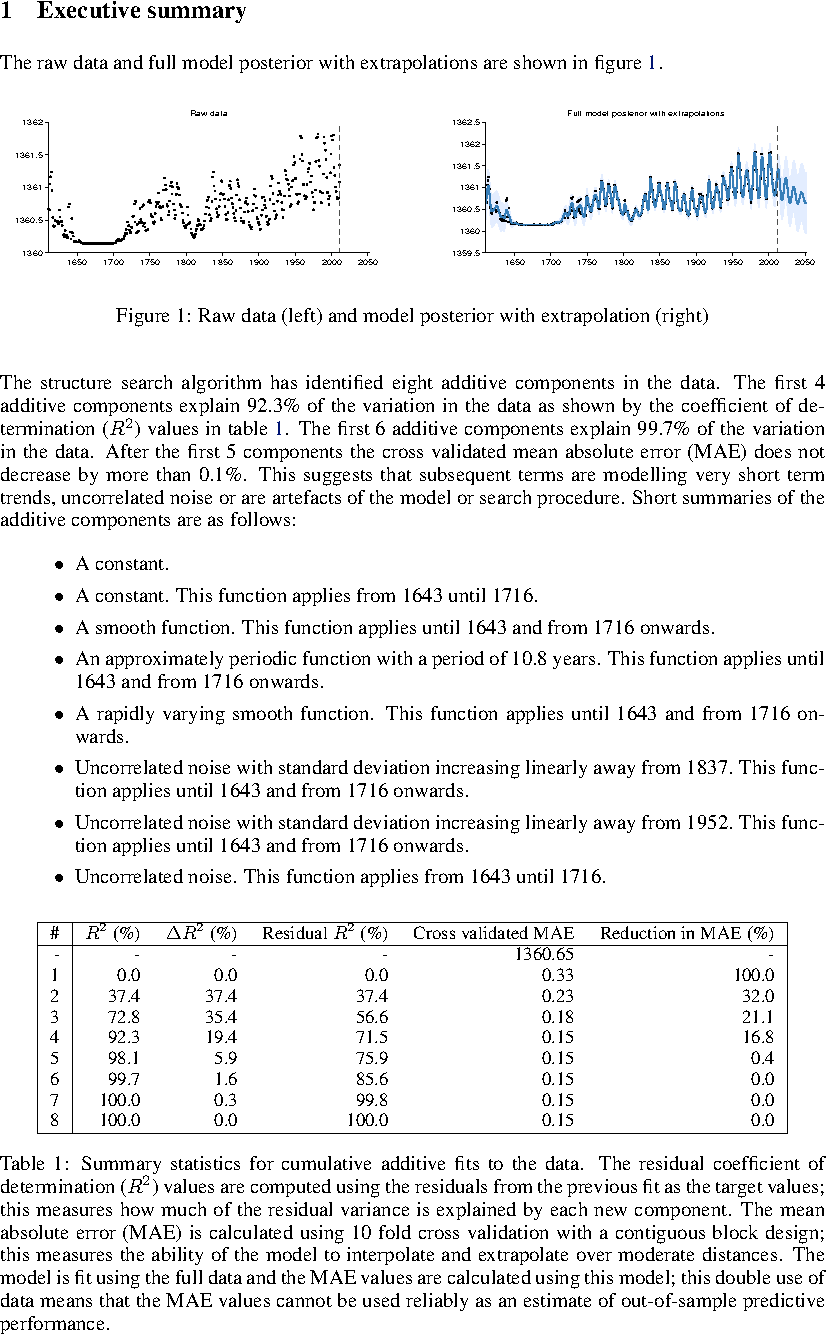
\includegraphics[trim=0.2cm 18.0cm 8cm 2cm, clip, width=0.98\columnwidth, height=0.45\columnwidth]{solarpages/pg_0002-crop}
\caption{
Solar irradiance data.}
\label{fig:solar}
\end{figure}

Here we show excerpts from the report automatically generated on annual solar irradiation data from 1610 to 2011 (figure~\ref{fig:solar}).
This time series has two pertinent features: a roughly 11-year cycle of solar activity, and a period lasting from 1645 to 1715 with much smaller variance than the rest of the dataset.  This flat region corresponds to the Maunder minimum, a period in which sunspots were extremely rare \citep{lean1995reconstruction}.
The \procedurename{} search procedure and automatic description clearly identify these two features, as discussed below.

After distributing and simplifying, the kernel corresponding to the first four components is as follows:
%\vspace{-0.5\baselineskip}
%\begin{itemize}
%  \itemsep0em
%  \item $\kC$
%  \item $\kCW(\emptyset,\kC)$
%  \item $\kCW(\kSE,\emptyset)$
%  \item $\kCW(\kSE \times \kPer,\emptyset).$
%\end{itemize}
%\vspace{-\baselineskip}
$\kC + \kCW(\emptyset,\kC) + \kCW(\kSE,\emptyset) + \kCW(\kSE \times \kPer,\emptyset).$


\begin{figure}[h]
\centering
\fbox{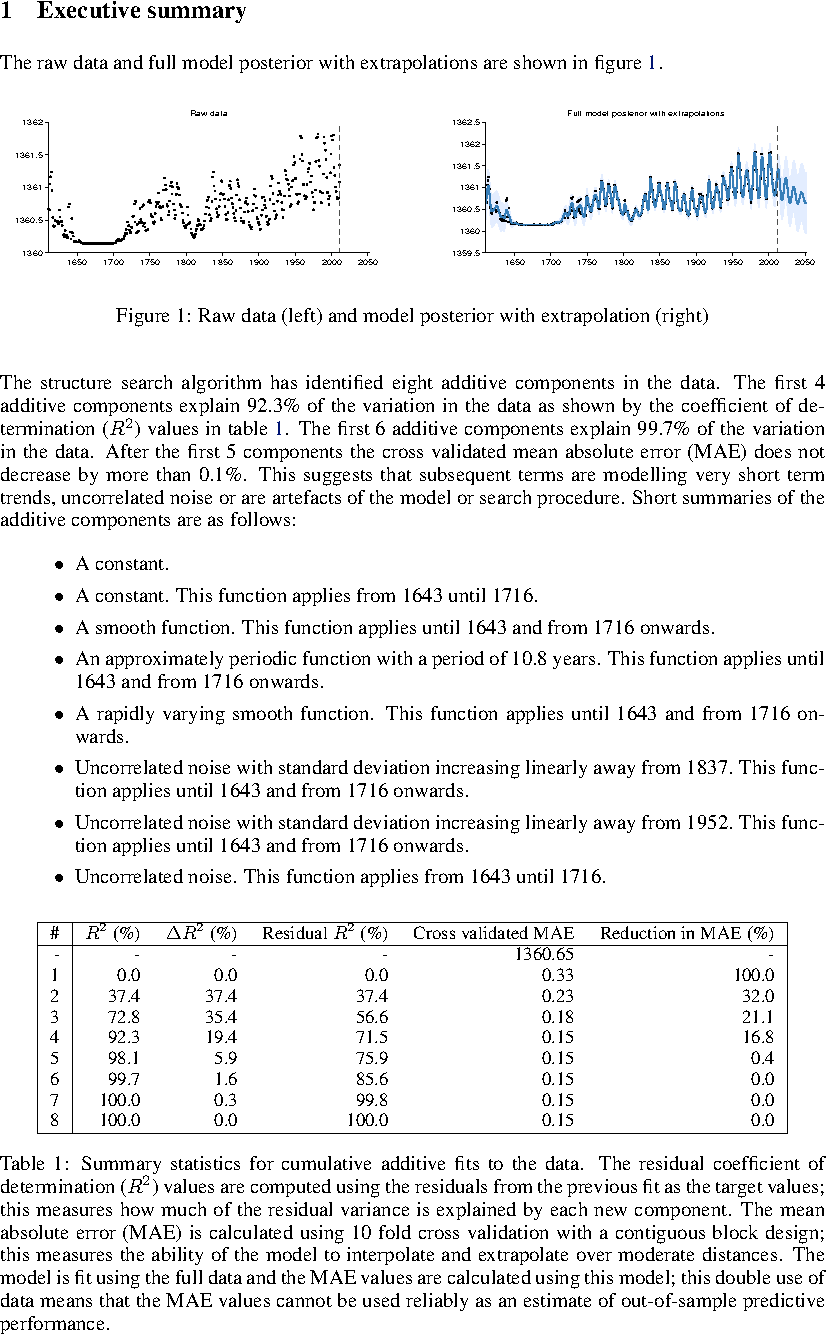
\includegraphics[trim=0cm 10.8cm 0cm 6.3cm, clip, width=0.98\columnwidth]{solarpages/pg_0002-crop}}
\caption{
An example of an automatically-generated summary of a dataset.  The dataset is decomposed into diverse structures with simple descriptions.}
\label{fig:exec}
\end{figure}
Figure \ref{fig:exec} shows the natural-language summaries of these components produced by \procedurename{}.
%The short descriptions demonstrate how the kernel is split into univariate enveloping functions (from the change windows) and stationary kernels.
%
%
%The model uses 9 additive components to explain the data, and reports that the first 4 components explain more than 90\% of the variance in the data.
%This might seem incongruous with the observation that there are two main features of the data, but if we examine the first four components, we see that the first component is describing the mean of the dataset, the second is the Maunder minimum, the third describes the long-term trend, and the fourth describes the 11-year periodicity.
From these short summaries, we can see that the model has identified the Maunder minimum (second component) and 11-year solar cycle (fourth component).
Next, we discuss each component in greater detail.
%This might seem incongruous with the observation that there are two main features of the data, but if we examine the first four components, we see that the first component is describing the mean of the dataset, the second is the Maunder minimum, the third describes the long-term trend, and the fourth describes the 11-year periodicity.

%\subsubsection{Signal versus Noise}
%
%One design challenge we encountered was seperating the recovered structure into signal and noise.  Originally, the model always included a term corresponding to \iid{} additive Gaussian noise.  However, in practice, the distinction between signal and noise is unclear for two reasons.  First, a component which varies arbitrarily quickly in time can be indistinguishable from noise.  Second, the variance of the noise may change over time (called heteroscedasticity), and this sort of pattern may be considered part of the signal.
%Because of the blurry distinction between signal and noise, we include a table which summarizes the relative contribution of each component in terms of held-out predictive power.%  To do this, we order the components in terms of how much each one improves predictive performance in a 10-fold cross-validation procedure.  The intuition for this metric is that noise-like components do not contribute much to the extrapolation performance of the model, but that signal-like components do.
%
%
%\begin{figure}
%\centering
%\fbox{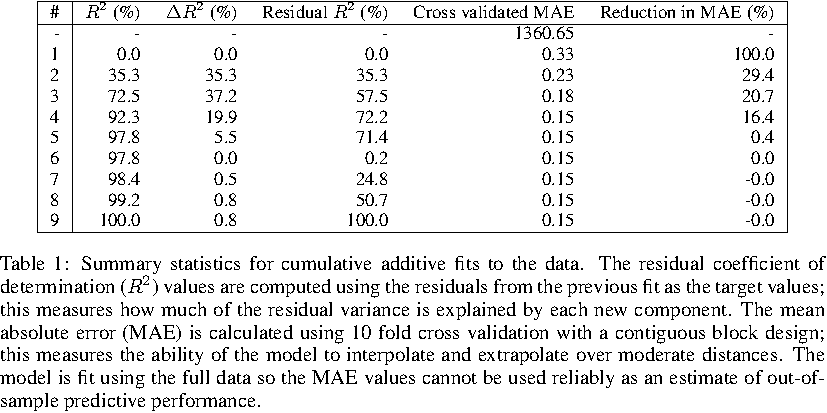
\includegraphics[width=0.98\columnwidth]{solarpages/02-solar-seperate-pages-3}}
%\caption{A table summarizing the relative contribution of the 9 different components of the model in terms of predictive performance.}
%\label{fig:table}
%\end{figure}
%
%Figure \ref{fig:table} show an example of this table on the solar dataset.

%Because the user may be interested in local or noisy components, we report all components to the user.  
%An interactive version of our procedure could allow users to specify which components are of interest, and group the remaining components into a single noise component.

%\paragraph{Decomposition plots}

%The second section of each report contains a detailed discussion of each component.
%Every component is plotted, and properties of the covariance structure are described.
%Some components are not meaningful when plotted on their own, so we also include plots of the cumulative sum of components.
%\paragraph{Automatic Plotting}
%The posterior of the individual component and sum of all components so far is visualised by plots of the posterior mean and variance.
%First, the posterior mean and variance of each component is plotted on its own.
%Second, the posterior mean and variance of all components shown so far is plotted against the data.
%This progression of plots 
%By contrasting each of these plots with plots of earlier components, we can see 
%shows qualitatively how each component contributes to an overall explanation of the data.

%A second paragraph explains the improvement in predictive performance gained by including this component in the model. This is the same informatino as included in the executive summary.

%\paragraph{Maunder minimum}

Figure \ref{fig:maunder} shows that \procedurename{} has captured the unusual period of decreased solar activity from about 1645 to 1715, and is able to report this in natural language.
%
\begin{figure}[ht]
\centering
\fbox{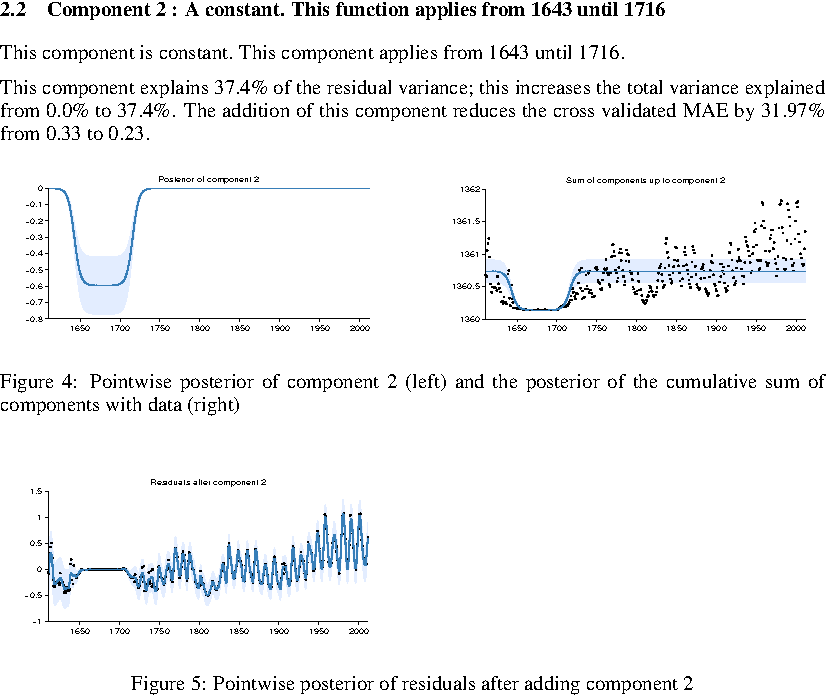
\includegraphics[trim=0cm 4.75cm 0cm 0.7cm, clip, width=0.98\columnwidth]{solarpages/pg_0005-crop}}
\caption{Discovering the Maunder minimum.}
\label{fig:maunder}
\end{figure}
%
%\paragraph{Long term trend}
%
Having isolated the Maunder minimum, the model captures the long-term trend of the rest of the data, shown in figure~\ref{fig:smooth}.
%
\begin{figure}[h!]
\centering
\fbox{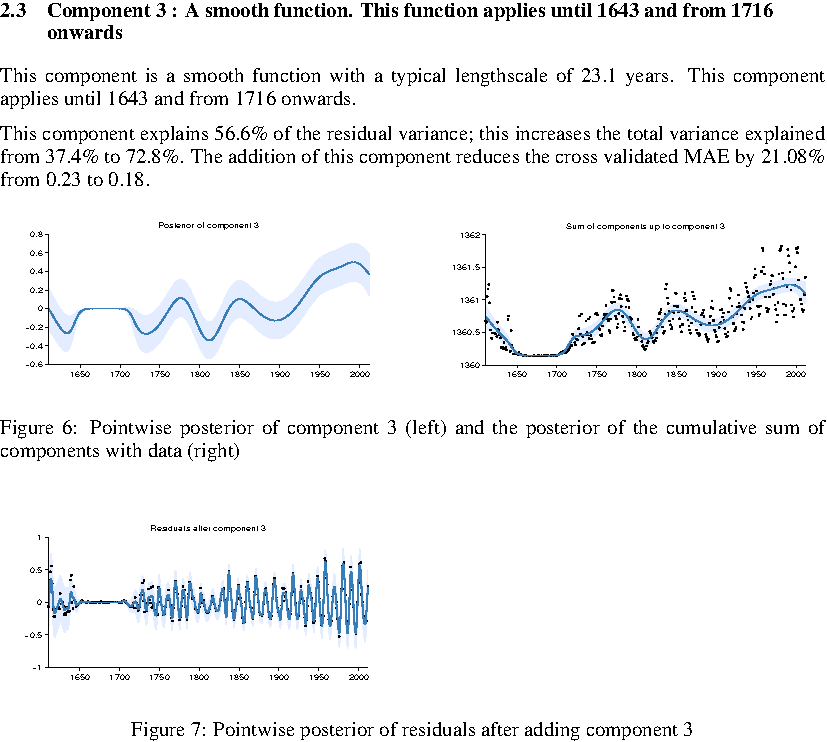
\includegraphics[trim=0cm 4.75cm 0cm 1cm, clip, width=0.98\columnwidth]{solarpages/pg_0006-crop}}
\caption{Characterizing the medium-term smoothness of solar activity levels.  By allowing other components to explain the periodicity, noise, and the Maunder minimum, \procedurename{} can isolate the part of the signal best explained by a slowly-varying trend.}
\label{fig:smooth}
\end{figure}
%
% is a good example of a meaningful component discovered by \procedurename, whose meaning would be unclear without an individual plot.  
%
%
%In the history of solar activity, the Maunder minimum is a good example of a local change in covariance.  Specifically, 
%The changepoint kernels used by \procedurename encode changes in covariance structure.
%For example, from about 1645 to 1715, solar activity decreased.
%, and very few sunspots were observed, a period called the Maunder Minimum \citep{lean1995reconstruction}.
%This feature was captured by the model by multiplying a constant kernel by two changepoint kernels.
%
%\paragraph{Solar cycles}
%
Figure \ref{fig:periodic} shows that \procedurename{} has isolated the approximately 11 year solar cycle.
By examining the parameters of the kernels comprising this component the description identifies that the shape of the periodicity is near sinusoidal and also quantifies how quickly the exact shape of the sinusoid changes.
%
%with a pair of changepoint kernels.%shows exactly which sort of structure was recovered by this component.
%
%\begin{figure}[h!]
%\centering
%\fbox{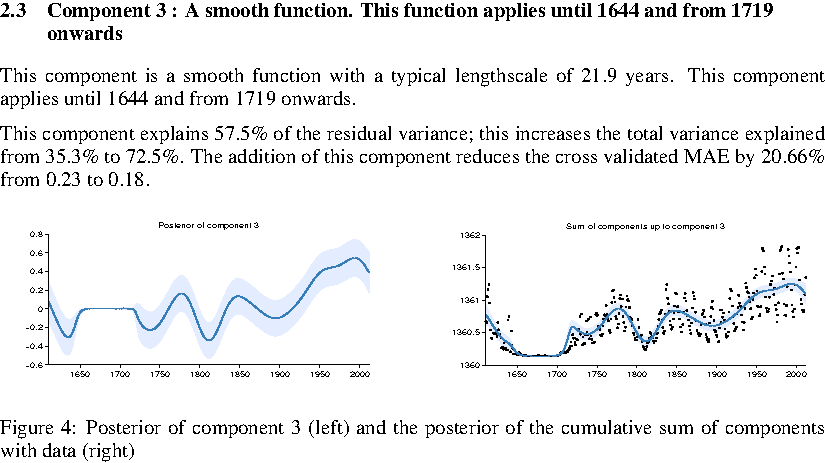
\includegraphics[width=0.98\columnwidth]{solarpages/02-solar-seperate-pages-6}}
%\caption{Characterizing the medium-term smoothness of solar activity levels.  By allowing other components to explain the periodicity, noise, and the Maunder minimum, we can isolate the part of the signal best explained by a slowly-varying trend.}
%\label{fig:smooth}
%\end{figure}
%
%\paragraph{Isolating the smoothly-varying component} Examining the dataset by eye, overall solar activity seems to change slowly over decades.  However, this intuition seems difficult to formalize.  Linear or quadratic regression is clearly inappropriate, and methods based on local smoothing would need to control for the periodic component.  Luckily, the \procedurename procedure does exactly this, allowing us to isolate the slowly-varying component of the data, without having to forecast either the Maunder minimum or the periodic variation.  Figure \ref{fig:smooth} shows the automatically-generated summary of this component.



%Figure \ref{fig:periodic} shows that \procedurename has identified the approximately 11 year solar cycle.
%By isolating this component in separate plots it is easy to see the exact nature of the solar cycle \eg how the amplitude of this periodic component varies over time.
%This demonstrates one benefit of isolating individual components: we can now see, by eye, extra structure that was not explicitly captured by the model.  Specifically, we can see that the amplitude of the periodic component varies over time.

%and by comparing with figure \ref{fig:smooth}, we can see that it varies roughly in proportion to the overall magnitude of the signal.
%  This pattern suggests that some sort of log-transform might be appropriate for this dataset, or that the model should be extended in some way to capture this structure.

%\paragraph{Extrapolation plots}
%
%The third section of each report shows extrapolations into the future, as well as posterior samples from each individual component of the model.  These samples help to characterize the uncertainty expressed by the model, and the extent to which different components contribute to predicting the future behavior of a time series.
%%
%The predictive mean and variance of the signals shown in the summary plots are useful, but do not capture the joint correlation structure in the posterior.  Showing posterior samples is a simple and universal way to illustrate joint statistical structure.
%%
%\begin{figure}[ht]
%\centering
%\fbox{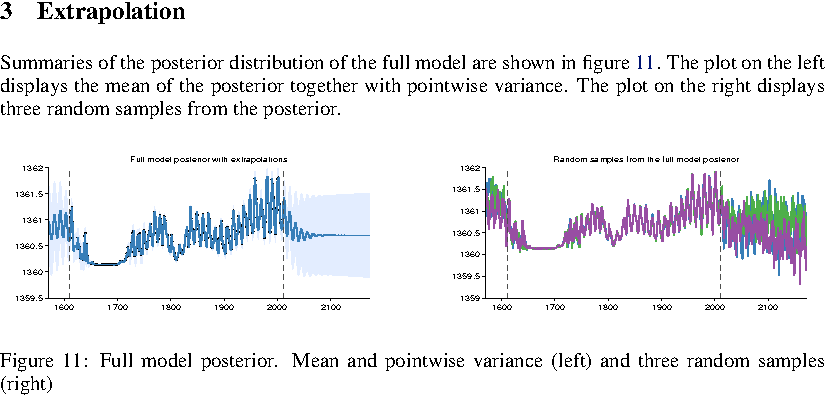
\includegraphics[trim=0cm 0cm 0cm 2.8cm, clip, width=0.98\columnwidth]{solarpages/02-solar-seperate-pages-13}}
%\caption{Sampling from the posterior.  These samples help show not just the predictive mean and variance, but also the predictive covariance structure.  Note, for example, that the predictive mean (left) does not exhibit periodicity, but the samples (right) do.}
%\label{fig:extrap-full}
%\end{figure}
%%
%For example,
%%  shows the predictive mean and variance given the entire model. 
%it is not clear from the left-hand plot in figure \ref{fig:extrap-full} whether or not the periodicity of the dataset is expected to continue into the future.  However, from the samples on the right-hand size, we can see that this is indeed the case.  

%\begin{figure}[h!]
%\centering
%\fbox{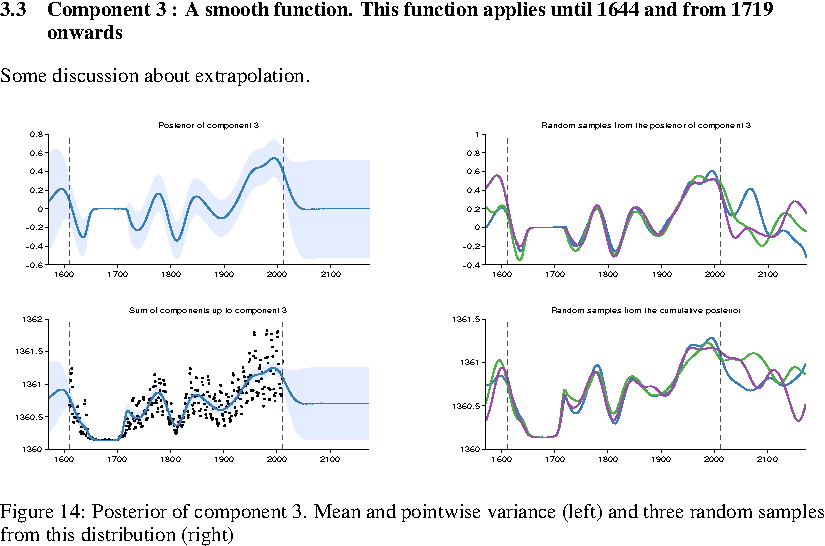
\includegraphics[width=0.98\columnwidth]{solarpages/02-solar-seperate-pages-16}}
%\caption{Extrapolating a single component of the model.  Because our model class allows us to isolate individual components, we can show the extent to which the model expects different trends to continue.  We also observe that the posterior samples are quite different from the posterior mean, away from the data.}
%\label{fig:extrap-smooth}
%\end{figure}

%\paragraph{Extrapolating individual components}
%We can also examine the model's expectations about the future behavior of individual components through sampling.  Further plots in the extrapolation section show posterior samples for each individual additive component. %For example, in figure \ref{fig:extrap-smooth}, we are shown samples of the predictive distribution of the smooth component of variation.  This plot indicates that the model considers a wide range of future average intensities to be plausible, but that it always expects those average intensities to vary smoothly.


\subsection{Describing heteroscedasticity}
\label{sec:airline}

\begin{figure}[h]
\centering
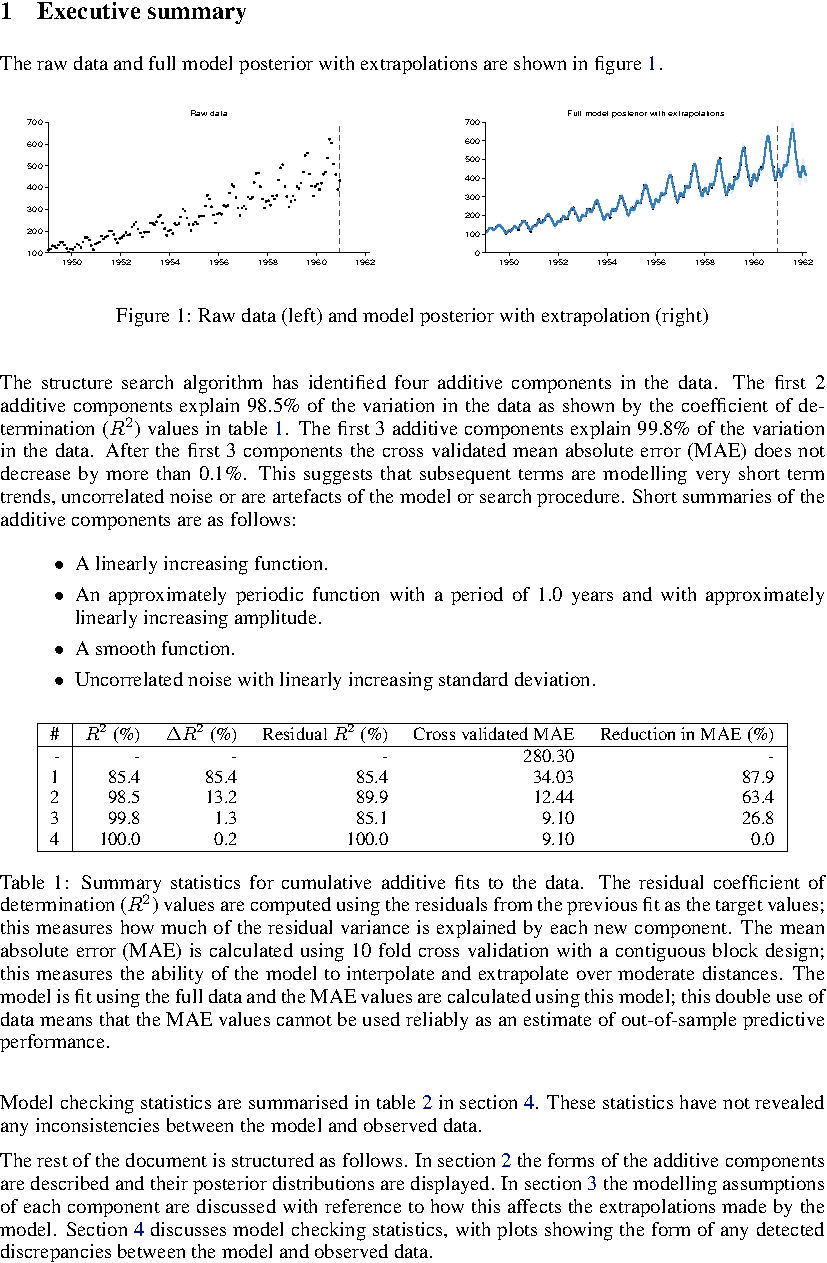
\includegraphics[trim=0.4cm 16.8cm 8cm 2cm, clip, width=0.98\columnwidth, height=0.45\columnwidth]{airlinepages/pg_0002-crop}
\caption{
International airline passenger data.}
\label{fig:airline}
\end{figure}

Next, we present the analysis generated by our procedure on international airline passenger data (figure~\ref{fig:airline}).
The model constructed by \procedurename{} has four components: $\kLin + \kSE \times \kPer \times \kLin + \kSE + \kWN \times \kLin$, with descriptions given in figure~\ref{fig:exec-airline}.
%\vspace{-0.5\baselineskip}
%\begin{itemize}
%  \itemsep0em
%  \item $\kSE$
%  \item $\kSE \times \kPer \times \kLin$
%  \item $\kSE$
%  \item $\kWN \times \kLin$
%\end{itemize}
%\vspace{-\baselineskip}
%
\begin{figure}[h]
\centering
\fbox{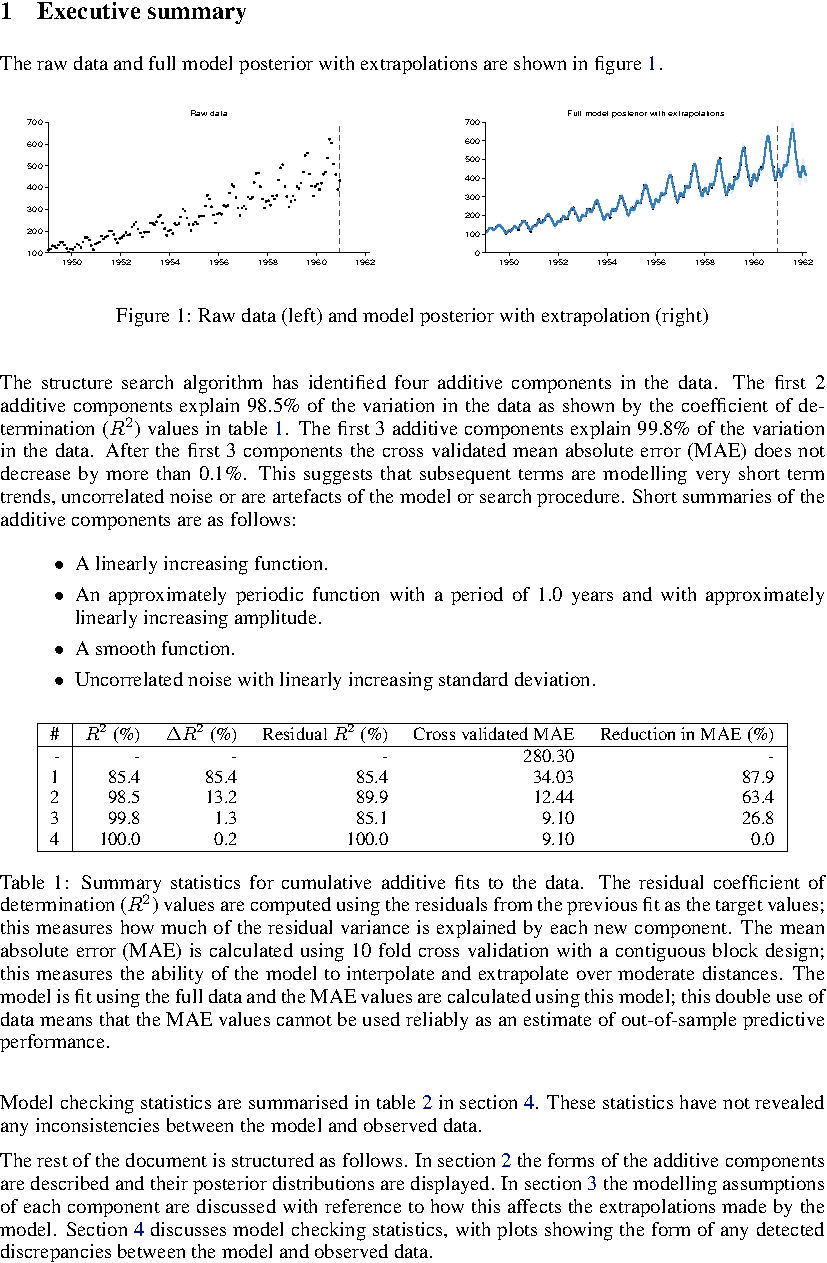
\includegraphics[trim=0cm 6.8cm 0cm 6cm, clip, width=0.98\columnwidth]{airlinepages/pg_0002-crop}}
\caption{
Short descriptions and summary statistics for the four components of the airline model.}
\label{fig:exec-airline}
\end{figure}
%
%\paragraph{Monotonic trend}
%\fTBD{JL: This will change to a linear trend in the official version - unless vetoed}
%No model in the current language can express a prior over monotonic functions.
%However, it is simple to check the posterior for monotonicity and remark upon it when appropriate (figure~\ref{fig:monotonic}).

%\begin{figure}[h]
%\centering
%\fbox{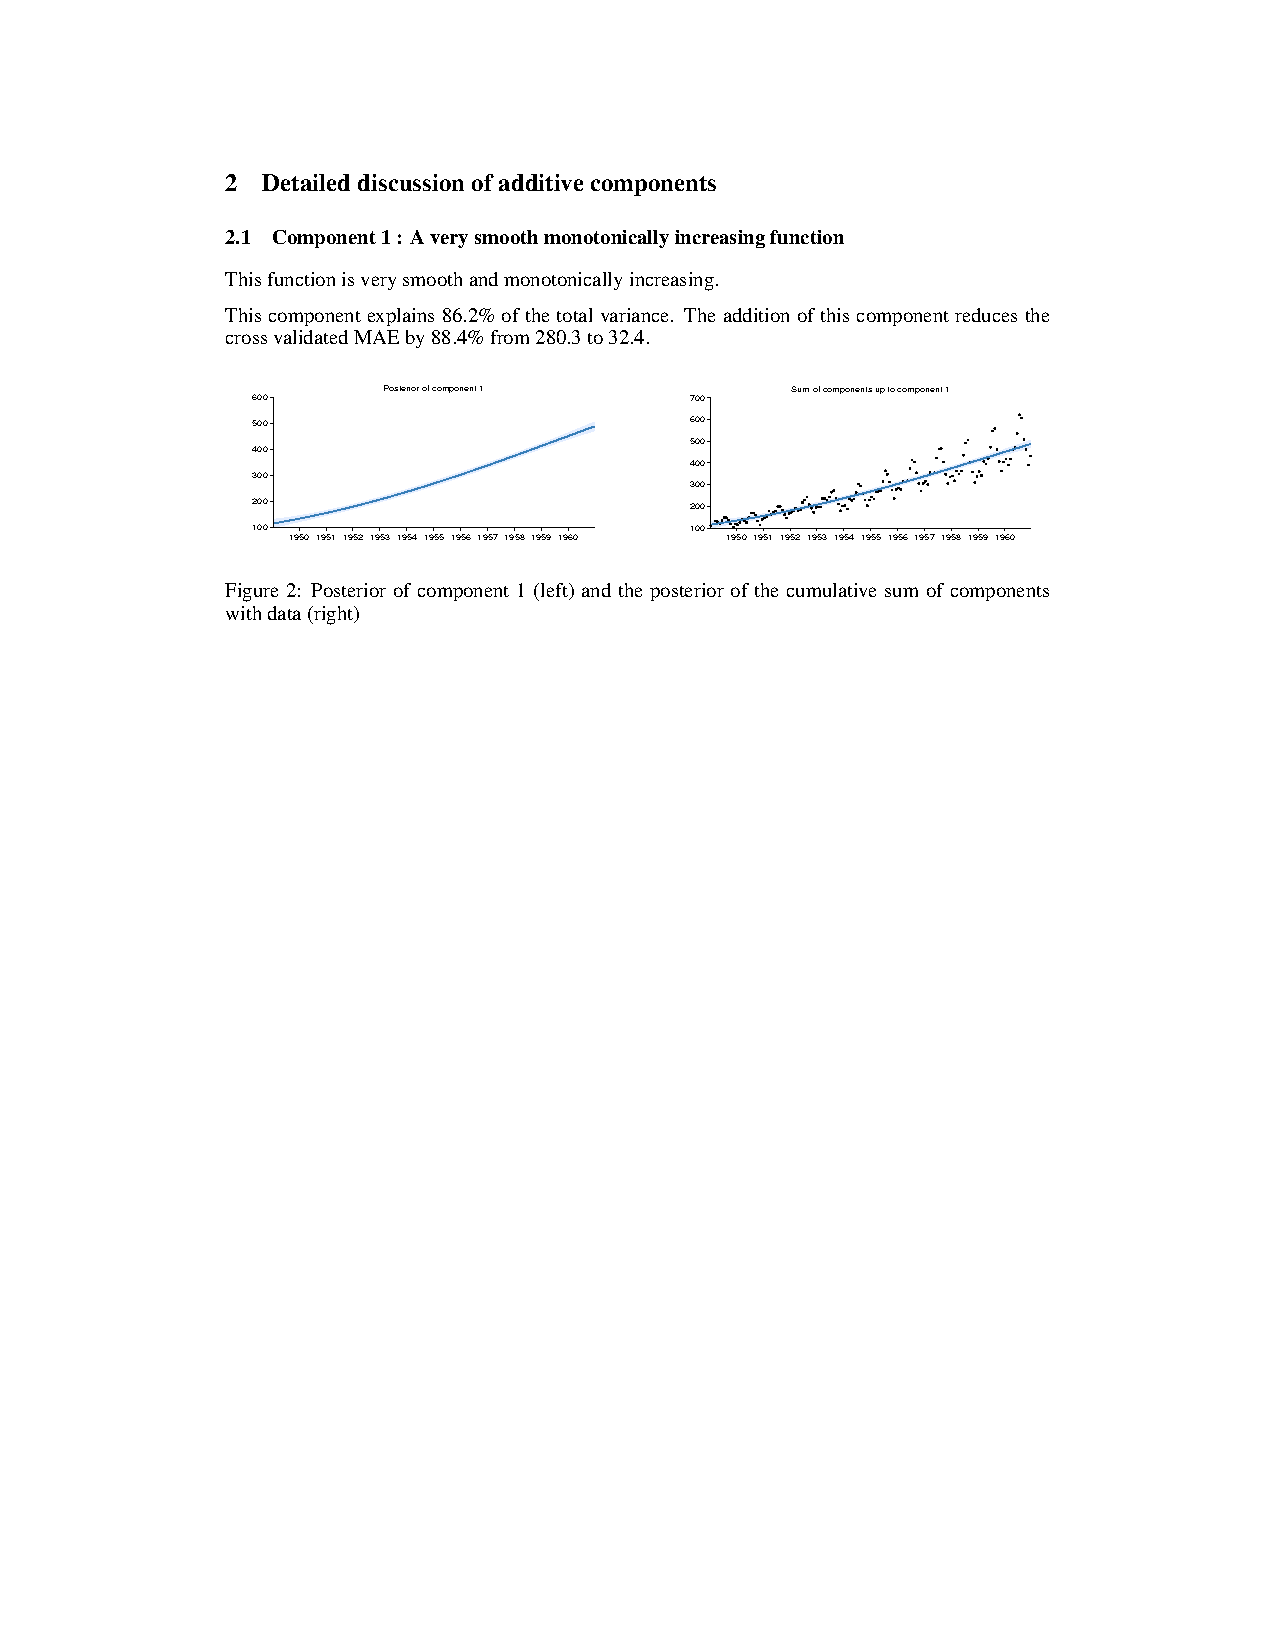
\includegraphics[trim=0cm 0cm 0cm 0cm, clip, width=0.98\columnwidth]{airlinepages/01-airline-separate-pages-3}}
%\caption{Describing monotonicity of the posterior}
%\label{fig:monotonic}
%\end{figure}

%\paragraph{Annual periodicity with linearly growing amplitude}

The second component (figure~\ref{fig:lin_periodic}) is correctly described as approximately ($\kSE$) periodic ($\kPer$) with linearly growing amplitude ($\kLin$).
%
\begin{figure}[h]
\centering
\fbox{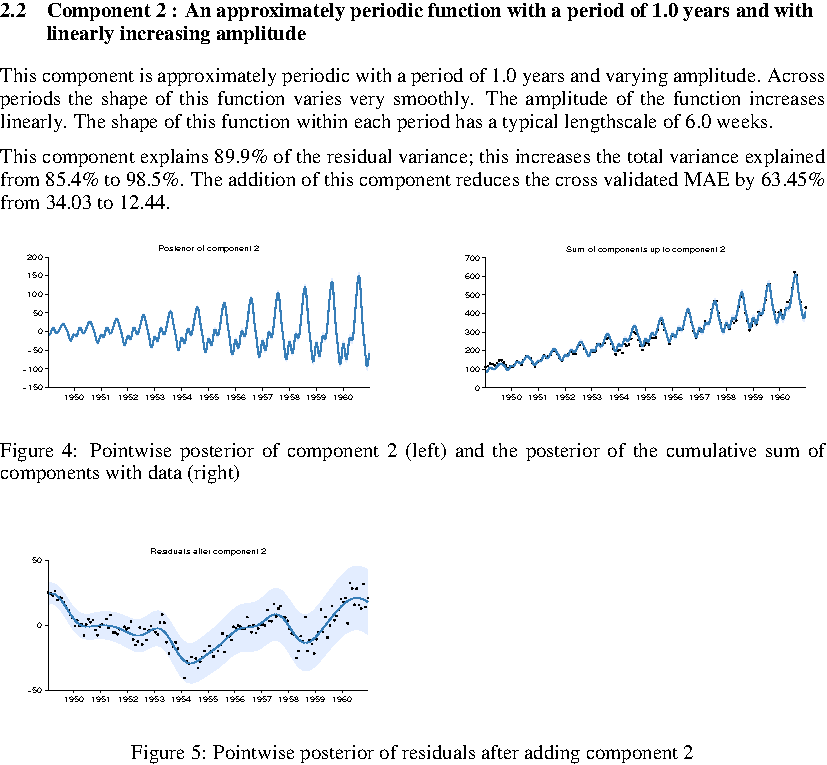
\includegraphics[trim=0cm 4.75cm 0cm 0cm, clip, width=0.98\columnwidth]{airlinepages/pg_0004-crop}}
\caption{Capturing non-stationary periodicity in the airline data}
\label{fig:lin_periodic}
\end{figure}
%
%\begin{figure}[h]
%\centering
%\fbox{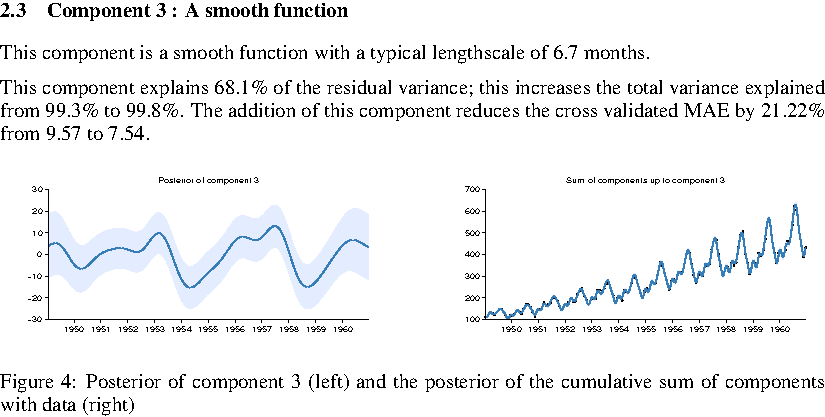
\includegraphics[trim=0cm 17cm 0cm 3.5cm, clip, width=0.98\columnwidth]{airlinepages/01-airline-separate-pages-5}}
%\caption{
%A caption.}
%\label{fig:exec}
%\end{figure}
%
%\paragraph{Linear heteroscedasticity}
%
By multiplying a white noise kernel by a linear kernel, the model is able to express heteroscedasticity (figure~\ref{fig:heteroscedastic}).
%
\begin{figure}[h]
\centering
\fbox{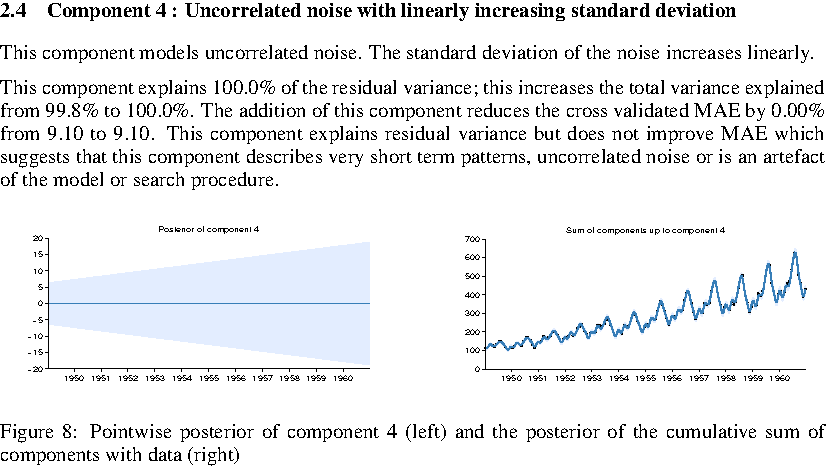
\includegraphics[trim=0cm 0cm 0cm 0cm, clip, width=0.98\columnwidth]{airlinepages/pg_0006-crop}}
\caption{Modelling heteroscedasticity}
\label{fig:heteroscedastic}
\end{figure}

\subsection{Comparison to equation learning}

%Much of machine learning research focuses on numerical performance, with claims of interpretability generated post-hoc.
%In contrast, equation learning \citep[e.g.][]{Schmidt2009b} can also be used to automate interpretation.

Eureqa \citep{Eureqa} is a system capable of producing parametric descriptions of time-series.
Here, we show equations produced by Eureqa for the data sets shown above, using the default mean absolute error performance metric.
%\footnotetext{We experimented with the root mean squared error with Akaike information criterion penalisation (analogous to the criterion used by \procedurename{}) but occasionally observed severe overfitting.}


The learned equation for the solar irradiance data is
\begin{align*}
\textrm{Irradiance($t$)} = 1361 + \alpha\sin(\beta + \gamma t)\sin(\delta + \epsilon t^2 - \zeta t)
\end{align*}
where $t$ is time (the input to the regression) and constants are replaced with symbols for brevity.
This equation captures the constant offset of the data, and models the long term trends with a product of sinusoids, but fails to capture the solar cycle or the Maunder-minimum.

The learned equation for the airline passenger data is
\begin{align*}
\textrm{Passengers($t$)} = \alpha t + \beta\cos(\gamma - \delta t)\textrm{logistic}(\epsilon t - \zeta) - \eta
\end{align*}
which captures the approximately linear trend, and the periodic component with approximately linearly (logistic) increasing amplitude.
However, the periodicity is heavily approximated with only a single sinusoid and the model cannot capture heteroscedasticity.





\section{Related work}
\label{sec:related-work}

\paragraph{Building Structured Covariance Functions}
\cite{rasmussen38gaussian} devote 4 pages to manually constructing a complex kernel to model the time series of Mauna Loa carbon dioxode conentrations over time.
A report automatically generated by \procedurename{} on this data set is included in the supplementary material and discovers a very similar model. 
Other examples of papers whose main contribution is to use domain knowledge to manually construct and fit a compound \gp{} kernel are \cite{klenske2012nonparametric} and \cite{lloydgefcom2012}.

\paragraph{Equation learning}

%In this work we have defined a search space of statistical models, where each model is characterised by a parametric covariance function.
%Previous work has considered searching over parametric functions \citep[e.g.][]{Schmidt2009b}.
%Some functions are well explained parametrically \eg a logistic function, whereas others are best described by their covariance \eg an approximately periodic function.
\cite{schmidt2009distilling}, \cite{todorovski1997declarative} and \cite{washio1999discovering} learn parametric forms of equations specifying time series, or relations between quantities.
In constrast, \procedurename{} learns a parametric form of the covariance allowing it to model functions without a simple parametric form.
%Because our system specifies the more general\fTBD{JL: Sounds like we are claiming we are a super set of equation learning - we need more kernels to make this claim} covariance structure rather than the functions themselves, we are able to capture structure which does not have a simple parametric form.

\paragraph{Searching over statistical models}

The line of work leading to \procedurename{} was originally inspired by the search over matrix factorisation models by \cite{grosse2012exploiting}.
Automatic model search is possible whenever the following conditions are met: 1) we can define a large space of models by combining a small number of components in a small number of different ways; 2) inference can be performed for all models in this space; 3) a basic search procedure is sufficient to find accurate models.
These conditions were also met for example in \citet{kemp2008discovery} who learned the structural form of a graph used to model human similarity judgments.  

More generally, probabilistic programming [cite]\fTBD{Is there a canonical reference yet \eg I don't think there are any books} software automatically generates inference mechanisms for open-ended classes of models, enabling automatic model search.
For example, \cite{VikashScene13} automatically searches over models of 2D scenes.
\fTBD{JL: Something about graphical models?}

%\NA{
%This is also true of - can we also cite some sort of graphical model work?
%}
%\fTBD{RG: Cite Kemp + Tenenbaum?}

%\paragraph{Standard inference methods}
%\fTBD{RG: How is this relevant?}
%The \procedurename language can express many regression motifs as \gp{}s for which inference is well understood.
%Probabilistic programming (cite) defines languages that describe generative models in such a way that %inference can be performed in each model.
%Extending the model search ideas in \procedurename to searches over probabilistic programs would be an interesting area for future research (cite Josh's workshop paper?).

\paragraph{Natural-language descriptions of data}

To the best of our knowledge, our procedure is the first example of automatic description of nonparametric statistical models.
However, grammar-based techniques have previously been used to automatically understand images \cite{zhu2007stochastic} and recently \citet{GanesalingamG13} produced a theorem proving system that expresses its proofs in natural language.

\subsection{Improvements to the previous grammar}

Our space of \gp{} models is closely based on that of \citet{DuvLloGroetal13}, with several improvements which yield more interpretable models. We briefly summarize the differences and the motivations for them:
\begin{itemize}
\item We added changepoint and window operators, which capture structure occuring only during certain time periods.
\item We introduced the white noise kernel ($\kWN$); combined with linear kernels or changepoints, this can produce heteroskedastic models, i.e.~ones with time-varying noise.
\item We added the constant kernel ($\kC$) explicitly, rather than implicitly adding a constant function to all kernels. This allows constant components to be reported separately.% in the reports.
\item We replaced the periodic kernel with a more flexible one which includes the cosine kernel as a limiting case. \citet{bochner1959lectures} demonstrated that any stationary kernel can be approximated as a sum of kernels of this form.
\end{itemize}




%\section{Numerical evaluation}
\section{Predictive Accuracy}
\label{sec:numerical}

To complement our demonstration of the interpretability of \procedurename{}, we compared the predictive accuracy of various model-building algorithms at interpolating and extrapolating time-series.
On these datasets, \procedurename{} on average outperforms the other methods.% on average (\eg as measured by quantiles of performance metrics).
%\NA{However, the variability of the results suggests that there is room to improve the robustness of \procedurename.}
%\fTBD{JL: I'm trying to avoid claims of oversell - any thoughts on a measured statement?}

\paragraph{Data sets}

In addition to the three time series analysed by \cite{DuvLloGroetal13} we evaluate the performance of the algorithms listed below on 10 additional time series from the time series data library \citep{TSDL}; plots of the data can be found at the beginning of the reports in the supplementary material\fTBD{Assuming all the reports fit within size constraints}.

\paragraph{Algorithms}

We compare the structure search algorithm to equation learning using Eureqa \citep{Eureqa} and six other regression algorithms; linear regression, \gp{} regression with a single $\kSE$ kernel (squared exponential), a Bayesian variant of multiple kernel learning \citep[e.g.][]{bach2004multiple}-, change point modelling (CP) / multi resolution Gaussian processes \citep[e.g.][]{garnett2010sequential, FoxDunson:NIPS2012}, spectral kernels (SP) \citep{WilAda13} and trend-cyclical-irregular (TCI) \citep[e.g.][]{lind2006basic}\fTBD{Can anyone find a more academic reference?}.

We use the default mean absolute error criterion when using Eureqa.
All other algorithms can be expressed as restrictions of our modelling language (see table~\ref{table:motifs}) so we perform inference using the same search methodology and selection criterion\footnotemark~(Bayesian information criterion) with appropriate restrictions to the grammar.
For MKL, trend-cyclical-irregular and spectral kernels this corresponds to a forward selection algorithm.
\footnotetext{We experimented with using unpenalised conditional likelihood as the search criterion for other methods but observed overfitting as is to be expected.} 

We restricted to regression algorithms for comparability; this excludes models which regress on previous values of times series \citep[e.g.][]{box2013time}.
Producing model construction algorithms for this class of time-series model would be an interesting area for future research.

\paragraph{Model Search and Inference}

As in \citep{DuvLloGroetal13}, \procedurename{} searched through models using a greedy search, using exact \gp{} inference to evaluate marginal likelihood, and conjugate gradient descent to optimize kernel parameters.
%In these experiments, \procedurename{} uses exact \gp{} inference,  \cite{DuvLloGroetal13} but we introduce new search operators to accommodate the changepoint and change window operators.
The search operators used are provided in the supplementary material.

\paragraph{Interpretability versus accuracy}

Since the process of describing a model always converts a kernel into a sum of products we experimented with always keeping the kernel in this form.
After applying search operators to a kernel we distributed all products over addition, changepoint and changewindow operators and simplified the resulting expression.
This variant (\procedurename{} interpretability) of the search tends to produce models with fewer additive components improving interpretability.
We also include the unrestricted version of the search (\procedurename{} accuracy) which tends to produce models that are better at extrapolation and interpolation.
%
%The research leading up to this manuscript has focused on interpretability.
%One could almost certainly improve the numerical results presented in this section by reintroducing $\kRQ$ and including Mat\'ern kernels as well as others.
We leave a full exploration of the interpretability / accuracy trade-off for future work.

\paragraph{Extrapolation}

To test extrapolation we trained all algorithms on the first 90\% of the data, and attempted to predict the remaining 10\% and then computed the root mean squared error (RMSE).
The RMSEs are then standardised by dividing by the smallest RMSE for each data set, so that the best performance on each data set will have a value of 1.
%
Figure~\ref{fig:box_extrap_dist} shows the standardised RMSEs across algorithms.
%Both versions of \procedurename{} have lower quartiles than all other methods but the outliers of \procedurename{}, TCI and SP have similar values.

\begin{figure*}[ht]
\centering
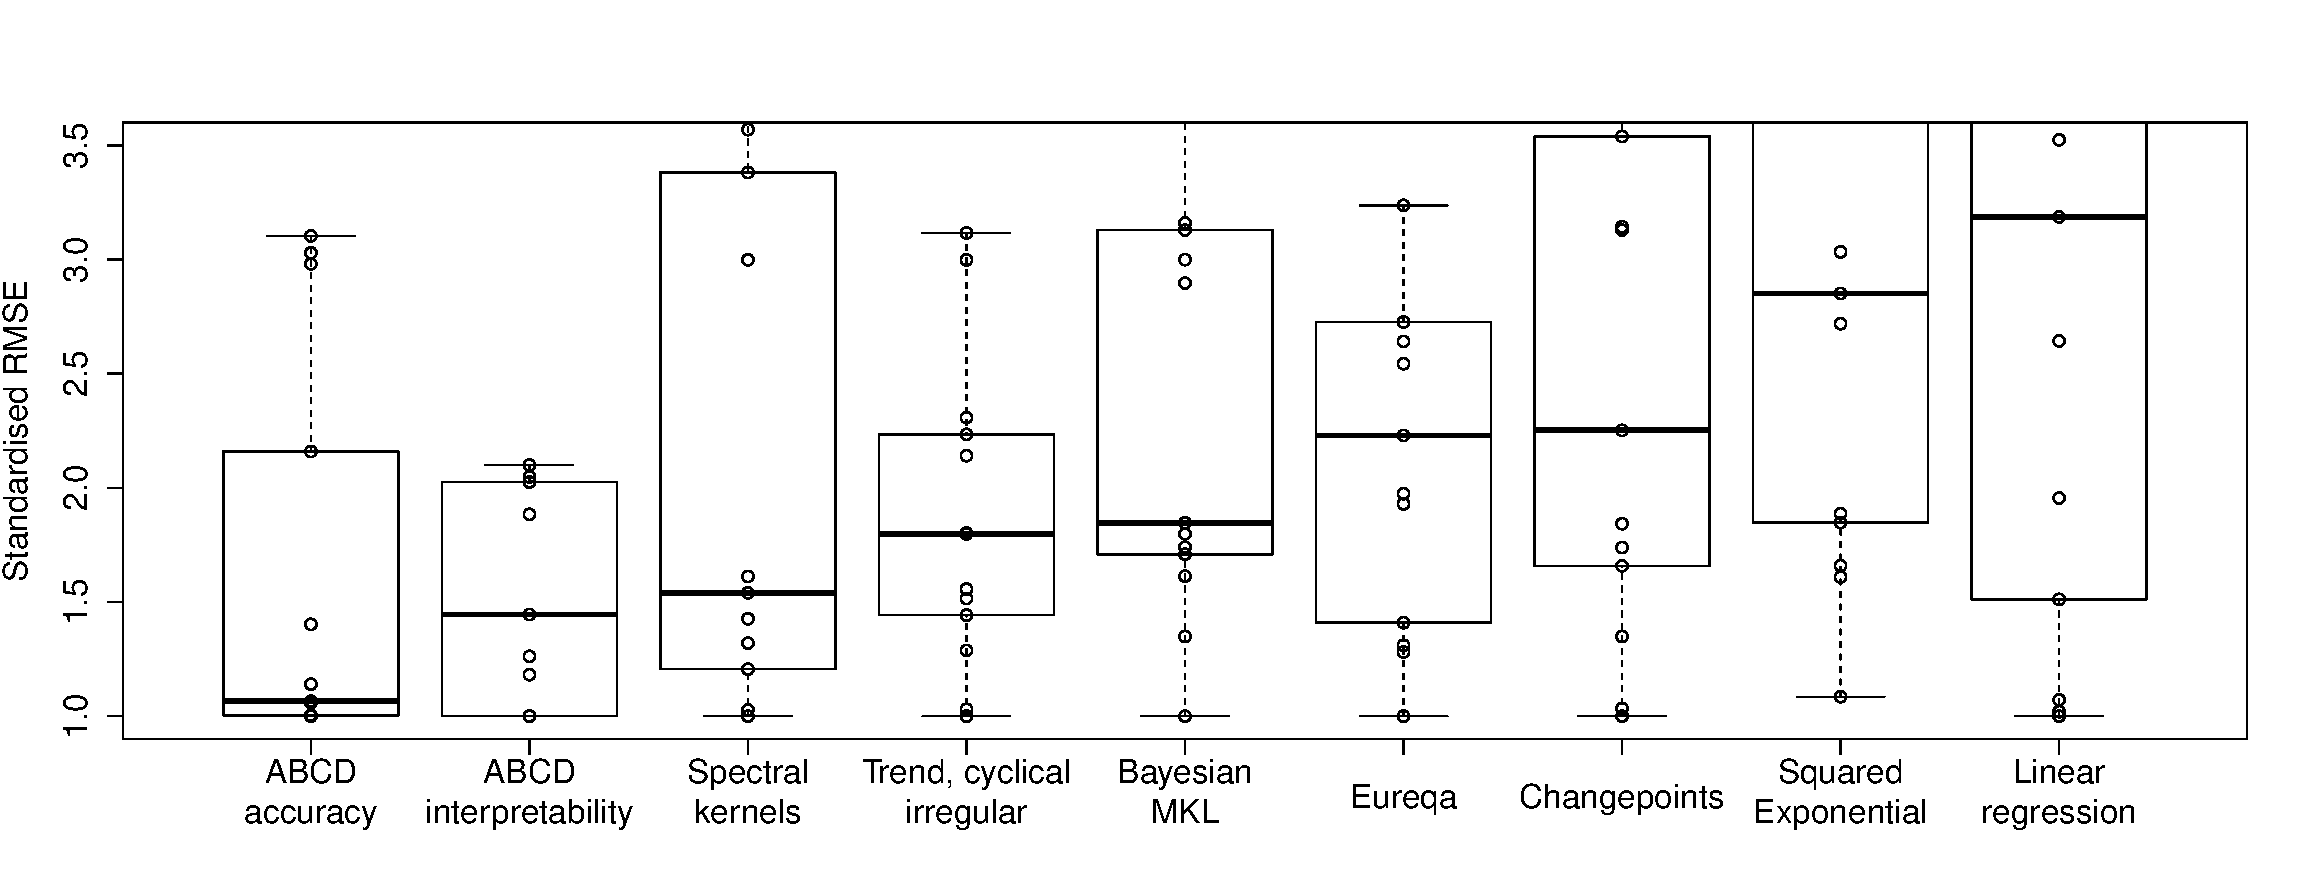
\includegraphics[width=\textwidth]{figures/box_extrap_wide}
\caption{
Raw data, and box plot of standardised extrapolation RMSE (best performance = 1).
Ordered by median.
}
\label{fig:box_extrap_dist}
\end{figure*}

Overall, the model construction methods with the greater capacity perform better: trend-cyclical-irregular outperforms Bayesian MKL, which outperforms squared exponential.
Eureqa performs relatively poorly, since very few datasets are well explained by a parametric equation.

Not shown on the plot are large outliers for spectral kernels, Eureqa, squared exponential and linear regression with values of 11, 493, 22 and 29 respectively.
All of these outliers occurred on a data set with a large and sharp discontinuity (see the call centre data in the supplementary material).
%All methods attempted to model this discontinuity using inappropriate components resulting in wild predictions.

%Also not shown on the plot is a very large outlier for EL of 493 (this was also on the call centre data).
%However, EL was the best performing algorithm on the wages dataset which shows an exponential increase after the industrial revolution.
%\procedurename can approximate an exponential function with a polynomial by combining $\kLin$ kernels but this is not a succinct expression in the current language.
%Expanding the modelling language of \procedurename is a natural area for future research.

%Somewhat surprisingly, TCI performs well despite its restrictive modelling assumptions (smooth functions and exact periodicity).
%Further inspection of the extrapolation has revealed that while TCI cannot model non-stationarity, its extrapolations of approximately periodic components can be quite effective.
%While \procedurename and SP will quickly become uncertain about a roughly periodic component, TCI will predict the average which is often more effective.
%This suggests that models composed of kernels of the form $(\kSE + \kC) \times \kPer$ will be effective for extrapolating approximately periodic components.

\paragraph{Interpolation}
To test the ability of the methods to interpolate, we randomly divided each data set into equal amounts of training data and testing data.
%We trained each algorithm on the training half of the data, produced predictions for the remaining half and then computed standardised RMSEs.
The results are similar to those for extrapolation, can be found in the supplementary material.





\section{Discussion}

Towards the goal of automating the process of statistical analysis we have introduced a system that can automatically construct and describe complex statistical models.
To the best of our knowledge this is the first system that can automatically describe any model in an open-ended class of nonparametric models in natural language.
We have also demonstrated that out procedure has competitive extrapolation and interpolation performance compared to other model construction techniques.

%Thinking towards extending this line of work many questions and challenges are raised which we briefly outline.

%\paragraph{Accuracy versus interpretability}
% DD: we already talk about this in the experimental section
%Typical machine learning research focuses on predictive performance rather than interpretability, likely due to the difficulty of assessing the interpretability of a method in an objective manner.
%Requiring that statistical models can be automatically described constrains the models that can be used over and above the traditional constraints of tractability.

%\paragraph{A sufficiently large class of models}
%To be non-trivial.

%\paragraph{Computational complexity}
%\fTBD{JL,DD: This can potentially be shortened - or even removed}
%\fTBD{JL: At the least it should not be a verbatim quote of JBT}
%\procedurename{} is embarassingly parallel, and can be run overnight on a cluster.
%This is computationally expensive compared to fitting only one or a small number of models.
%However, this computational cost may be reasonable when compared to the cost of having a human researcher iteratively propose, fit, and refine a series of models, especially when one considers the size and scope of the space of models that is searched, and the fact that all steps of model construction, evaluation and search are automatic.

%In our experience, working statisticians, machine learners, and data scientists rarely if ever explore such a space so systematically, partly because of the cost in terms of both their own time and computation time.
%The artificial intellgience presented in this paper is still quite primitive and naive, and the space of models we can consider automatically is still quite limited compared to what humans can do.
%However, in evaluating the limitations of these methods, and prospects for future work of this sort, other factors might loom larger than computational efficiency.



%\paragraph{Automatic description of methods}



%\paragraph{When is a description of a model useful as a description of data?}

%\fTBD{Shorten me significantly}

%\procedurename produces models, $M$, of the form $f = \sum_i f_i$ where $f_i \dist \gp{}(0, \kernel_i)$.
%The form of $M$ is chosen to be that which best explains observations of $f$, denoted by $D$, as measured by approximate marginal likelihood.

%In the reports generated by \procedurename, we show plots of the posterior $p(f_i^*\given M,D)$ but the natural-language descriptions are of typical elements of the prior $p(f_i^*\given M)$ given the fitted model \ie they are descriptions of the model rather than descriptions of the data.

%Despite fitting the model to the data by maximising the marginal likelihood $p(D\given M)$ the selected model may be a poor description of the data if the data contains features not easily expressed by the language of models defined by \procedurename.
%To test for when this is the case we have begun experimenting with posterior predictive checks to assess the models produced by \procedurename following the techniques of \cite{Gelman1996} (see reports in the supplementary material).
%In fact, the posterior predictive checks take the form of comparing the expectation of statistics under the prior and posterior of each component \ie they are testing whether or not typical elements of the posterior $p(f_i^*\given M,D)$ are typical elements of $p(f_i^*\given M)$.

%However, model checking for Gaussian processes, even those with simple kernels, is under-researched so we leave their description and more detailed analysis for future work. 

%\paragraph{Other systems}
%The system presented in this paper is just one example of a system combining these elements, for performing supervised regression.
%\citep{grosse2012exploiting} provides an earlier example with builds unsupervised models.
%Similar systems could be constructed in other learning scenarios, such as sequence modeling or semi-supervised learning.

\paragraph{Source Code}
Source code to perform all experiments is available on github, available upon publication.
%\href{http://www.github.com/jamesrobertlloyd/gpss-research}
%{\texttt{github.com/jamesrobertlloyd/gpss-research}}}
%All \gp{} hyperparameter tuning was performed by automated calls to the GPML toolbox\footnote{Available at 
%\href{http://www.gaussianprocess.org/gpml/code/}
%{\texttt{www.gaussianprocess.org/gpml/code/}}
%}

%\section{Discussion}

%\begin{quotation}
%``The availability of 'user-friendly' statistical software has caused authors to become increasingly careless about the logic of interpreting their results, and to rely uncritically on computer output, often using the 'default option' when something a little different (usually, but not always, a little more complicated) is correct, or at least more appropriate.''
% In trying to practice this art, the Bayesian has the advantage because his formal apparatus already developed gives him a clearer picture of what to expect, and therefore a sharper perception for recognizing the unexpected.

%\defcitealias{dyke1997avoid}{G. Dyke, 1997}
%\hspace*{\fill}\citet{Jaynes85highlyinformative}
%\hspace*{\fill}\citetalias{dyke1997avoid}
%\end{quotation}

%In this paper, we exhibited the output of a method for automatically constructing and summarizing a compositional Gaussian process regression model in natural language.
%These summaries can enable human experts and non-experts to understand the implications of a model, check its plausibility, and notice structure not yet captured by the model.

\bibliography{gpss}
\bibliographystyle{format/icml2014}

\end{document} 
